% Detailed algebra and boundary contracts moved from the main narrative.
% Labels are retained so all proof dependencies remain explicit.
\section{Detailed local algebra and information boundaries}
\label{sec:detailed-algebra}

\subsection{Frame action and unique alignments}
\begin{lemma}[Frame action]
\label{lem:frame-action}
Let \(u\) be a frame of length \(k\), let \(p,q\in S_k\), and let \(r\) be an
injective relabeling of references.  Then
\[
  \operatorname{id}\cdot u=u,
  \qquad
  p\cdot(q\cdot u)=(q\circ p)\cdot u
  =(q\mathbin{\mathrm{then}}p)\cdot u,
  \qquad
  r(p\cdot u)=p\cdot(ru).
\]
Hence Eq.~\eqref{eq:action} is a right action of \(S_k\) on frames, the orbit
\([u]_\Gamma=\{\gamma\cdot u:\gamma\in\Gamma\}\) is well defined for every
subgroup \(\Gamma\leq S_k\), and two witnesses are sequenced by
\(p\mathbin{\mathrm{then}}q\):
\((p\mathbin{\mathrm{then}}q)\cdot u=q\cdot(p\cdot u)\).
\end{lemma}

\begin{proof}
Coordinatewise,
\((p\cdot(q\cdot u))_i=(q\cdot u)_{p(i)}=u_{q(p(i))}=((q\circ p)\cdot u)_i\),
which is the stated anti-homomorphism law and is exactly the convention
\(p\mathbin{\mathrm{then}}q=p\circ q\) of the slot images.  Thus the
\code{then} API sequences tuple reorderings, although slot-map composition
has the reverse order from composition of those reorderings.  A relabeling acts on the values held by
the slots and the group acts on the slots themselves, so
\((r(p\cdot u))_i=r(u_{p(i)})=(ru)_{p(i)}=(p\cdot(ru))_i\).  Injectivity of
\(p\cdot u\) and of \(ru\) is inherited from \(u\) and \(r\).
\end{proof}

\begin{lemma}[Unique alignment]
\label{lem:unique-alignment}
Let \(u\) and \(v\) be frames of length \(k\) with
\(\operatorname{im}u=\operatorname{im}v\).  Then there is exactly one
\(\rho\in S_k\) with \(v=\rho\cdot u\), namely \(\rho=u^{-1}\circ v\).  In
particular every subgroup \(\Gamma\leq S_k\) acts freely on frames, so all
orbits have cardinality \(|\Gamma|\).
\end{lemma}

\begin{proof}
Both tuples are bijections onto the same image, so \(\rho=u^{-1}\circ v\) is a
permutation of slots and \((\rho\cdot u)_i=u_{\rho(i)}=v_i\).  If
\(v=\rho'\cdot u\) as well, then \(u_{\rho(i)}=u_{\rho'(i)}\) for every \(i\),
and injectivity of \(u\) forces \(\rho=\rho'\).  Freeness is the case
\(v=u\), which yields \(\rho=\operatorname{id}\), and the orbit--stabilizer
theorem then gives \(|[u]_\Gamma|=|\Gamma|\).
\end{proof}

The tetrahedral case is the smallest instance of this local state model.  Four
distinct ligand references admit \(4!=24\) frames, on which \(S_4\) acts freely
and transitively; the subgroup \(A_4\) has index two, so the frames split into
two orbits of twelve.  Even permutations are rigid rotations of one local
configuration and odd permutations reach the mirror orbit.

\begin{proposition}[Local parity criterion]
\label{prop:local-parity}
Let \(u\) and \(v\) be tetrahedral frames with
\(\operatorname{im}u=\operatorname{im}v\), and let \(\rho\in S_4\) be the unique
alignment of Lemma~\ref{lem:unique-alignment}, \(v=\rho\cdot u\).  Then
\[
 [u]_{A_4}=[v]_{A_4}
 \quad\Longleftrightarrow\quad
 \operatorname{sgn}(\rho)=+1 .
\]
If \(\operatorname{sgn}(\rho)=-1\), the two frames lie in the two distinct
cosets of \(A_4\) in \(S_4\).
\end{proposition}

\begin{proof}
By Lemma~\ref{lem:unique-alignment} the alignment \(\rho\) exists and is unique,
so \([u]_{A_4}=[v]_{A_4}\) holds precisely when \(\rho\in A_4\).  The sign
homomorphism \(\operatorname{sgn}:S_4\to\{\pm1\}\) has kernel \(A_4\), whence
\(\rho\in A_4\) is equivalent to \(\operatorname{sgn}(\rho)=+1\).  Since
\([S_4:A_4]=2\), every odd alignment lies in the unique remaining coset and
therefore reaches the opposite orbit.
\end{proof}


\subsection{Focal-configuration-neutral carrier perception}
\label{sec:perception-algorithm}

Perception produces typed \emph{potential} elements, not configured
descriptors.  Let \(\mathcal F\) be an optional set of supplied oriented frames
at other loci.  The focal frame is removed before its carrier is assessed, and
all CIP properties, coordinates, canonical local descriptors, and atom indices
are excluded.  Algorithm~\ref{alg:perception} makes this boundary explicit.

\begin{definition}[Potential-carrier predicate]
\label{def:potential-carrier}
For a family policy \(P\), identity profile \(\chi\), type \(\tau\), and
candidate support \(s\), let
\[
  \operatorname{Pot}_{\tau,P}(G_\chi,s;\mathcal F_{-s})
\]
mean that \(s\) is a structurally valid support of type \(\tau\) and passes
the registered configuration-neutral feasibility test.  The returned evidence
record is
\[
  e_s=(s,\tau,A_s,q_s,r_s,\bot,\textsc{unassessed}),
\]
where \(A_s\) is the action induced by the support stabilizer
\(\operatorname{Aut}_\chi(G,\mathcal F_{-s})_s\), \(q_s\) is the potential-carrier status,
\(r_s\) is its reason, \(\bot\) denotes absent configuration, and the final
field records that configurational persistence has not been assessed.
\end{definition}

The predicate is deliberately an over-approximation of experimentally
persistent stereochemistry.  It asserts neither a handedness nor a molecular
chirality verdict.  Its mathematical requirement is equivariance: if
\(f\in\operatorname{Iso}_\chi(G,H)\), then
\begin{equation}
  \operatorname{Pot}_{\tau,P}(G_\chi,s;\mathcal F_{-s})
  \Longleftrightarrow
  \operatorname{Pot}_{\tau,P}(H_\chi,f(s);f\mathcal F_{-s}),
  \qquad
  f_*A_sf_*^{-1}=A_{f(s)} .
  \label{eq:perception-equivariance}
\end{equation}

\begin{algorithm}[htbp]
\caption{Focal-configuration-neutral stereo-carrier perception}
\label{alg:perception}
\begin{algorithmic}[1]
\Require LLG \(G\), identity profile \(\chi\), optional neighboring frames \(\mathcal F\), family policy \(P\)
\Ensure Equivariant potential-element evidence with no focal configuration; serialization order is not identity
\State \(G_0 \gets \Call{EraseDerivedAndConfiguredState}{G_\chi}\)
\State \(\mathcal C \gets \Call{EnumerateTypedSupports}{G_0,P}\)
\State \(\mathcal E \gets [\,]\)
\ForAll{\(s\in\Call{CanonicalSupportOrder}{\mathcal C}\)}
  \If{\(\neg\Call{ValidateSupport}{G_0,s}\)}
    \State \(\mathcal E\gets\mathcal E\mathbin{\|}(s,\textsc{rejected},\textsc{invalid support})\)
    \State \textbf{continue}
  \EndIf
  \State \(\mathcal F_{-s}\gets\Call{RemoveFocalFrame}{\mathcal F,s}\)
  \State \(G_s\gets\Call{AddNeighborFrameConstraints}{G_0,\mathcal F_{-s}}\)
  \State \(A_s\gets\Call{InducedStabilizerAction}{\operatorname{Aut}(G_s)_s}\)
  \State \((q,r)\gets\Call{ConfirmCarrier}{\operatorname{type}(s),G_s,s,A_s}\)
  \State \(\mathcal E\gets\mathcal E\mathbin{\|}(s,q,r,\bot,\textsc{unassessed})\)
\EndFor
\State \Return \(\mathcal E\)
\end{algorithmic}
\end{algorithm}

\begin{proposition}[Perception soundness]
\label{prop:perception-soundness}
Assume every registered support enumerator, validator, and family confirmation
test is invariant under \(\chi\)-isomorphism transporting the supplied
neighboring frame constraints. Algorithm~\ref{alg:perception}
is then equivariant in the sense of Eq.~\eqref{eq:perception-equivariance}.
Its output contains no configuration that could depend on atom numbering,
CIP priority, or the focal input orientation.
\end{proposition}

\begin{proof}
Support enumeration and validation commute with \(f\) by assumption.
Conjugation by \(f\) maps
\(\operatorname{Aut}_\chi(G_s)_s\) onto
\(\operatorname{Aut}_\chi(H_{f(s)})_{f(s)}\), hence maps the induced slot
action and every invariant confirmation result onto its counterpart.
Canonical support ordering changes only output order.  The focal orientation
and all derived naming data were erased, and the algorithm writes \(\bot\) in
every configuration field.
\end{proof}

\(\Call{ConfirmCarrier}{}\) is geometry specific.  A tetrahedral support is
confirmed exactly when its center-stabilizer action contains no odd
permutation of the four coordination slots.  Planar-bond and axis candidates
require non-exchangeable terminal reference pairs under the support
stabilizer.  Coordination carriers require a declared shape with valid arity.
Path and plane carriers require their respective topology or authorized
sidecar contract.  Failed criteria retain the broad candidate with a structured
reason such as \code{symmetry\_related}.  They do not imply a molecular
achirality verdict.  The output configuration is always \(\bot\), and stability
is always unassessed.

Terminal-reference equivalence must also remain separate from the orbit of a
whole configured axis. A constitutional map can exchange both terminal pairs
simultaneously, preserving axial orientation. Such a map supplies terminal
equivalence witnesses without identifying a configured state with its mirror.
The independent coupled-terminal regression checks this distinction. Exact
configured-graph comparison retains the full joint frame action; a
\code{symmetry\_related} carrier reason alone cannot replace that comparison.

\subsection{Authorized attachment and completeness boundaries}
\label{sec:attachment}

Perception and configuration attachment are separate typed operations.
Let \(\mathcal D\) be a finite collection of evidence records, let
\(\operatorname{src}(d)\) identify their provenance, and let
\(\operatorname{Auth}\subseteq\mathcal D\) be the records whose source is an
explicit stereo encoding, a validated geometry, or a declared sidecar.
Authorization is transported with the evidence record: for an isomorphism
\(f\), the target evidence collection and authorized subset are
\(f\mathcal D\) and \(f\operatorname{Auth}\). Authorization and typing
are not recomputed from atom indices. Every support validator invoked below
must satisfy the same profile-relative invariance contract as perception.

\begin{definition}[Authorized attachment]
\label{def:attachment}
Attachment is the partial map
\[
  \operatorname{att}\colon(\mathcal X,d)\longmapsto
  \bigl(G,\ \mathcal R\cup\{s_d\}\bigr),
\]
defined exactly when the typing predicate \(\operatorname{Typed}(d,\mathcal
X)\) holds, that is, when
\(d\in\operatorname{Auth}\); the support of \(d\) is a perceived or declared
locus of the type \(\tau\) that \(d\) declares; the ports of \(d\) coincide with
\(P_s\) including owner scope for virtual references; the arity agrees with
\(k_\tau\); the supplied state is a \(\Gamma_\tau\)-orbit of an admissible frame
in the sense of Definition~\ref{def:admissible-frames}; and \(\mathcal R\)
carries no conflicting configuration at that locus.  If any conjunct fails,
\(\operatorname{att}\) is undefined and \(\mathcal X\) is returned unchanged
together with a structured refusal.
\end{definition}

\begin{lemma}[Attachment is equivariant and fail-closed]
\label{lem:attachment}
For every \(f\in\operatorname{Iso}_\chi(G,H)\),
\(\operatorname{Typed}(d,\mathcal X)\) holds if and only if
\(\operatorname{Typed}(f d,f\mathcal X)\) holds, and in that case
\(\operatorname{att}(f\mathcal X,f d)=f\operatorname{att}(\mathcal X,d)\).
Attaching the same configuration twice is idempotent, no undefined case
modifies \(\mathcal R\), and connectivity-only evidence, having
\(d\notin\operatorname{Auth}\), can never select a configuration orbit.
\end{lemma}

\begin{proof}
Every conjunct of \(\operatorname{Typed}\) is stated in terms of type, support,
ports, arity, and orbit membership, all of which are transported by \(f\); the
orbit condition is preserved because \(f\) acts on references and commutes with
the slot action by Lemma~\ref{lem:frame-action}.  The image locus is therefore
defined precisely when the source locus is, and the two constructions agree.
Idempotence holds because \(\mathcal R\cup\{s_d\}\) is a set union and the
conflict conjunct rejects any second, different state at the same locus.  The
remaining claims are immediate from the definition, which modifies
\(\mathcal R\) only on the defined branch.
\end{proof}

\begin{definition}[Support boundary and audit]
\label{def:support-boundary}
A \emph{support boundary} \(B\) is an invariant rule specifying which
configured loci must be represented for the requested claim.  Important
instances are \(B_{\mathrm{decl}}\), which contains exactly the source-declared
configured loci, and \(B_{\mathrm{strict}}\), which contains all supported
potential loci required by the active family policy.  The third instance is
\(B_{\mathrm{comp}}\), the population of supported configurations considered
by topology completion.  The audit
\[
  \operatorname{Audit}_{B}(G_\chi,\mathcal E,\mathcal R)
  \in\{\textsc{complete},\textsc{incomplete},\textsc{unsupported}\}
\]
returns \textsc{complete} exactly when every locus required by \(B\) has one
well-typed supported configuration and no required locus has unresolved or
unsupported semantics.
\end{definition}

Thus a binary verdict under \(B_{\mathrm{decl}}\) is a claim about the
represented source-declared stereograph.  It becomes a claim about every
supported stereogenic locus of the molecular input only under
\(B_{\mathrm{strict}}\).  Stating \(B\) prevents those two scientifically
different conclusions from being conflated.


\subsection{Finite-frame configuration orbits}
\label{sec:local-orbits}

For a finite geometry \(t\), a local frame \(u\) is an ordered tuple of anchors
and ligand references in the sense of Section~\ref{sec:representation}, and its
fixed configuration is the orbit
\[
  [u]_{\Gamma_t}=\{\gamma\cdot u:\gamma\in\Gamma_t\}.
\]
The stored local state is the orbit, not a preferred tuple.  An unspecified
orientation uses a larger information group
\(\Gamma_t^\uparrow\), but this does not enlarge equality of a specified
configuration.

Two groups act on the slots of a locus and must be distinguished.  The larger
one records which slot rearrangements are admissible at all; the smaller one
records which of them leave the configuration fixed.

\begin{definition}[Frame symmetry, admissible frames, geometry group]
\label{def:admissible-frames}
Let \(t\) be a finite geometry of arity \(k_t\).  The \emph{frame symmetry
group} \(\Sigma_t\leq S_{k_t}\) is the group of slot permutations compatible
with the port structure of \(t\).  For an atom-supported geometry every ligand
may occupy every coordination slot, so \(\Sigma_t=S_{k_t}\).  For the bond- and
axis-supported families the slots consist of two terminal pairs together with
their anchors, and \(\Sigma_t\) is the order-eight group generated by the two
within-end exchanges and the end exchange that carries the anchors with it.
The \emph{admissible frames} of a locus with frame \(u\) are
\(\operatorname{Fr}_t(u)=\Sigma_t\cdot u\), and the geometry-preserving group is
a subgroup \(\Gamma_t\leq\Sigma_t\).
\end{definition}

\begin{proposition}[Configuration count]
\label{prop:config-count}
Let \(u\) be an admissible frame of a geometry \(t\).  The assignment
\[
  \sigma\Gamma_t\;\longmapsto\;[\sigma\cdot u]_{\Gamma_t}
\]
is a bijection from the left-coset space \(\Sigma_t/\Gamma_t\) onto the set of
configurations of the locus.  The number of configurations is therefore the
index \([\Sigma_t:\Gamma_t]=|\Sigma_t|/|\Gamma_t|\), independently of the
representative \(u\).
\end{proposition}

\begin{proof}
By construction \(\Sigma_t\) acts transitively on \(\operatorname{Fr}_t(u)\),
and by Lemma~\ref{lem:unique-alignment} it acts freely, so
\(\sigma\mapsto\sigma\cdot u\) is a bijection
\(\Sigma_t\to\operatorname{Fr}_t(u)\).  Lemma~\ref{lem:frame-action} gives
\[
  \Gamma_t\cdot(\sigma\cdot u)
  =\{(\sigma\circ\gamma)\cdot u:\gamma\in\Gamma_t\}
  =(\sigma\Gamma_t)\cdot u ,
\]
so this bijection carries left cosets of \(\Gamma_t\) exactly onto
\(\Gamma_t\)-orbits.  Counting cosets gives the index, and a different
representative \(u'=\sigma_0\cdot u\) only translates the coset labels.
\end{proof}

Proposition~\ref{prop:config-count} reproduces the state counts of
Table~\ref{tab:center-types} without case analysis:
\(24/12=2\) tetrahedral, \(24/8=3\) square planar, \(120/6=20\) trigonal
bipyramidal, \(720/24=30\) octahedral, and \(8/4=2\) for the planar bond, the
atrop axis, and the cumulene axis. It distinguishes a unique binary opposite
from a mirror operation that requires additional registered geometric structure.

\begin{corollary}[Binary opposite]
\label{cor:binary-opposite}
If \([\Sigma_t:\Gamma_t]=2\), then \(\Gamma_t\trianglelefteq\Sigma_t\),
\(\Sigma_t/\Gamma_t\cong\mathbb Z/2\), and
\[
  \operatorname{opp}([u]_{\Gamma_t})=[\mu\cdot u]_{\Gamma_t},
  \qquad \mu\in\Sigma_t\setminus\Gamma_t ,
\]
is independent of the choice of \(\mu\) and satisfies
\(\operatorname{opp}\circ\operatorname{opp}=\operatorname{id}\).  If
\([\Sigma_t:\Gamma_t]>2\), the index alone selects no unique other state;
an additional normalizer or improper geometric action can still define a
mirror involution.
\end{corollary}

\begin{proof}
A subgroup of index two is normal and its quotient is the two-element group.
All elements of \(\Sigma_t\setminus\Gamma_t\) form the single nontrivial coset,
so \([\mu\cdot u]\) does not depend on \(\mu\), and applying the nontrivial
coset twice returns the trivial one.  When the index exceeds two, the quotient
set has more than one other state, so the index-two uniqueness argument no
longer applies. This does not exclude additional invariant structure: an
element \(\mu\in N_{\Sigma_t}(\Gamma_t)\) with
\(\mu^2\in\Gamma_t\) induces a well-defined involution
\([u]\mapsto[\mu\cdot u]\). The registered TBP and octahedral improper
actions are examples despite their indices 20 and 30.
\end{proof}

For tetrahedral geometry \(\Sigma_t/\Gamma_t\) is the sign quotient
\(S_4/A_4\), so Corollary~\ref{cor:binary-opposite} specializes to
Proposition~\ref{prop:local-parity}.  The same index-two argument applies to the
planar bond and to both axis families.  A configuration-changing permutation at
a square-planar, trigonal-bipyramidal, or octahedral center is by contrast a
general reconfiguration in the local relation API. Its separately registered
geometric mirror may nevertheless supply an involution.  Figure~\ref{fig:orbit-examples} gives
one representative move per atom- or bond-supported geometry; full orbit
enumerations are given in Appendix~\ref{sec:si-orbits}.

\begin{figure*}[htbp]
  \centering
  \resizebox{\textwidth}{!}{% Representative permutation and relation class for each of the six geometries.
% Input-only TikZ file; requires concept_style.tex (Okabe--Ito palette, \iosub).
% Paul Tol qualitative ligand colors (colorblind-safe).
\providecolor{pballA}{RGB}{68,119,170}
\providecolor{pballB}{RGB}{238,119,51}
\providecolor{pballC}{RGB}{34,136,51}
\providecolor{pballD}{RGB}{170,51,119}
\providecolor{pballE}{RGB}{102,204,238}
\providecolor{pballF}{RGB}{221,204,68}

\begin{tikzpicture}[
  font=\small,
  gball/.style={circle, draw=black!30, minimum size=4.4mm, inner sep=0pt},
  slotn/.style={font=\tiny, text=black!55, inner sep=0.6pt},
  gbond/.style={line width=0.7pt, black!60},
  catom/.style={circle, draw=black!55, fill=white, minimum size=3.6mm,
                inner sep=0pt, font=\tiny},
  perm/.style={-{Latex[length=1.9mm]}, line width=0.7pt, black!55},
  vopp/.style={rounded corners=2pt, draw=ioBlue!55!black, fill=ioBlue!10,
               font=\scriptsize\bfseries, text=ioBlue!45!black, inner sep=2.4pt},
  vrec/.style={rounded corners=2pt, draw=ioOrange!70!black, fill=ioOrange!18,
               font=\scriptsize\bfseries, text=ioOrange!45!black, inner sep=2.4pt},
  veq/.style={rounded corners=2pt, draw=ioGreen!60!black, fill=ioGreen!14,
              font=\scriptsize\bfseries, text=ioGreen!45!black, inner sep=2.4pt}
]

% ---- shape drawers: center (cx,cy) + ligand colors in slot order ----------
% \ghl draws the specular highlight that turns a flat disc into a 3D sphere
\newcommand{\ghl}[2]{\fill[white,opacity=0.12] ({#1-0.07},{#2+0.07}) circle (0.066);}
\newcommand{\tetF}[6]{\begin{scope}[shift={(#1,#2)}]
  \coordinate (o) at (0,0);
  \foreach \p/\c in {{(0,0.60)}/#3,{(0.62,-0.05)}/#4,{(-0.55,-0.55)}/#5,{(0.45,-0.62)}/#6}
    \draw[gbond] (o) -- \p;
  \fill[black] (o) circle (0.045);
  \node[gball,fill=#3] at (0,0.60){}; \node[gball,fill=#4] at (0.62,-0.05){};
  \node[gball,fill=#5] at (-0.55,-0.55){}; \node[gball,fill=#6] at (0.45,-0.62){};
  \ghl{0}{0.60}\ghl{0.62}{-0.05}\ghl{-0.55}{-0.55}\ghl{0.45}{-0.62}
  \node[slotn] at (-0.16,0.74){1}; \node[slotn] at (0.80,0.02){2};
  \node[slotn] at (-0.72,-0.62){3}; \node[slotn] at (0.62,-0.72){4};
\end{scope}}
\newcommand{\sqF}[6]{\begin{scope}[shift={(#1,#2)}]
  \coordinate (o) at (0,0);
  \foreach \p in {(0,0.66),(0.66,0),(0,-0.66),(-0.66,0)} \draw[gbond] (o)--\p;
  \fill[black] (o) circle (0.045);
  \node[gball,fill=#3] at (0,0.66){}; \node[gball,fill=#4] at (0.66,0){};
  \node[gball,fill=#5] at (0,-0.66){}; \node[gball,fill=#6] at (-0.66,0){};
  \ghl{0}{0.66}\ghl{0.66}{0}\ghl{0}{-0.66}\ghl{-0.66}{0}
  \node[slotn] at (-0.18,0.78){1}; \node[slotn] at (0.80,0.14){2};
  \node[slotn] at (-0.18,-0.78){3}; \node[slotn] at (-0.80,0.14){4};
\end{scope}}
\newcommand{\tbpF}[7]{\begin{scope}[shift={(#1,#2)}]
  \coordinate (o) at (0,0);
  \foreach \p in {(0,0.80),(0,-0.80),(-0.72,0.05),(0.72,0.20),(0.58,-0.34)}
    \draw[gbond] (o)--\p;
  \fill[black] (o) circle (0.045);
  \node[gball,fill=#3] at (0,0.80){}; \node[gball,fill=#4] at (0,-0.80){};
  \node[gball,fill=#5] at (-0.72,0.05){}; \node[gball,fill=#6] at (0.72,0.20){};
  \node[gball,fill=#7] at (0.58,-0.34){};
  \ghl{0}{0.80}\ghl{0}{-0.80}\ghl{-0.72}{0.05}\ghl{0.72}{0.20}\ghl{0.58}{-0.34}
  \node[slotn] at (0.20,0.86){1}; \node[slotn] at (0.20,-0.86){2};
  \node[slotn] at (-0.86,0.14){3}; \node[slotn] at (0.86,0.30){4};
  \node[slotn] at (0.72,-0.42){5};
\end{scope}}
\newcommand{\octF}[8]{\begin{scope}[shift={(#1,#2)}]
  \coordinate (o) at (0,0);
  \foreach \p in {(-0.52,0.30),(0.52,0.30),(0.52,-0.30),(-0.52,-0.30),(0,0.82),(0,-0.82)}
    \draw[gbond] (o)--\p;
  \fill[black] (o) circle (0.045);
  \node[gball,fill=#3] at (-0.52,0.30){}; \node[gball,fill=#4] at (0.52,0.30){};
  \node[gball,fill=#5] at (0.52,-0.30){}; \node[gball,fill=#6] at (-0.52,-0.30){};
  \node[gball,fill=#7] at (0,0.82){}; \node[gball,fill=#8] at (0,-0.82){};
  \ghl{-0.52}{0.30}\ghl{0.52}{0.30}\ghl{0.52}{-0.30}\ghl{-0.52}{-0.30}\ghl{0}{0.82}\ghl{0}{-0.82}
  \node[slotn] at (-0.66,0.44){1}; \node[slotn] at (0.66,0.44){2};
  \node[slotn] at (0.66,-0.44){3}; \node[slotn] at (-0.66,-0.44){4};
  \node[slotn] at (0.18,0.90){5}; \node[slotn] at (0.18,-0.90){6};
\end{scope}}
% bond frame: two centers, 2 substituents each end. #7 = 1 (double) or 0 (single/twist)
\newcommand{\bondF}[7]{\begin{scope}[shift={(#1,#2)}]
  \coordinate (cL) at (-0.40,0); \coordinate (cR) at (0.40,0);
  \ifnum#7=1
    \draw[gbond] (-0.40,0.05)--(0.40,0.05); \draw[gbond] (-0.40,-0.05)--(0.40,-0.05);
    \def\dy{0.52}
  \else
    \draw[gbond] (cL)--(cR); \def\dy{0.34}
  \fi
  \draw[gbond] (cL)--(-0.92,\dy); \draw[gbond] (cL)--(-0.92,-\dy);
  \draw[gbond] (cR)--(0.92,\dy);  \draw[gbond] (cR)--(0.92,-\dy);
  \node[catom] at (cL){C}; \node[catom] at (cR){C};
  \node[gball,fill=#3] at (-0.92,\dy){}; \node[gball,fill=#4] at (-0.92,-\dy){};
  \node[gball,fill=#5] at (0.92,\dy){};  \node[gball,fill=#6] at (0.92,-\dy){};
  \ghl{-0.92}{\dy}\ghl{-0.92}{-\dy}\ghl{0.92}{\dy}\ghl{0.92}{-\dy}
  \node[slotn] at (-1.10,\dy){1}; \node[slotn] at (-1.10,-\dy){2};
  \node[slotn] at (1.10,\dy){5};  \node[slotn] at (1.10,-\dy){6};
\end{scope}}

% ---- generic panel arrow + verdict ----------------------------------------
\newcommand{\panelarrow}[3]{% (x,y) plabel
  \draw[perm] (#1,#2) -- ++(1.25,0);
  \node[slotn, text=black!70] at (#1+0.62,#2+0.22) {#3};}

% ============================ Panels ======================================
% A Tetrahedral: swap two ligands -> OPPOSITE
\begin{scope}[shift={(0,0)}]
  \iosub[{$|\Sigma|{=}24$, $|\Gamma|{=}12$, $[\Sigma{:}\Gamma]{=}2$}]{-0.42,0.30}{A}{Tetrahedral \;\;$\Gamma_{\mathrm{tet}}{=}A_4$}
  \tetF{1.35}{-1.75}{pballA}{pballB}{pballC}{pballD}
  \panelarrow{2.55}{-1.75}{$\pi{=}(1\,2)$}
  \tetF{5.15}{-1.75}{pballB}{pballA}{pballC}{pballD}
  \node[vopp] at (3.55,-3.30) {OPPOSITE \;{\normalfont\scriptsize $\pi\notin\Gamma$, $[\Sigma{:}\Gamma]{=}2$}};
\end{scope}
% B Square planar: adjacent swap -> RECONFIGURED
\begin{scope}[shift={(8.40,0)}]
  \iosub[{$|\Sigma|{=}24$, $|\Gamma|{=}8$, $[\Sigma{:}\Gamma]{=}3$}]{-0.42,0.30}{B}{Square planar \;\;$\Gamma{=}D_4$}
  \sqF{1.35}{-1.75}{pballA}{pballB}{pballC}{pballD}
  \panelarrow{2.55}{-1.75}{$\pi{=}(1\,2)$}
  \sqF{5.15}{-1.75}{pballB}{pballA}{pballC}{pballD}
  \node[vrec] at (3.55,-3.30) {RECONFIGURED \;{\normalfont\scriptsize $\pi\notin\Gamma$, $[\Sigma{:}\Gamma]{>}2$}};
\end{scope}
% C Trigonal bipyramidal: axial<->equatorial -> RECONFIGURED
\begin{scope}[shift={(0,-4.60)}]
  \iosub[{$|\Sigma|{=}120$, $|\Gamma|{=}6$, $[\Sigma{:}\Gamma]{=}20$}]{-0.42,0.30}{C}{Trigonal bipyramidal \;\;$\Gamma{=}D_3$}
  \tbpF{1.35}{-1.75}{pballA}{pballB}{pballC}{pballD}{pballE}
  \panelarrow{2.55}{-1.75}{$\pi{=}(1\,3)$}
  \tbpF{5.15}{-1.75}{pballC}{pballB}{pballA}{pballD}{pballE}
  \node[vrec] at (3.55,-3.30) {RECONFIGURED \;{\normalfont\scriptsize $\mathrm{ax}\leftrightarrow\mathrm{eq}$, $[\Sigma{:}\Gamma]{=}20$}};
\end{scope}
% D Octahedral: cis swap -> RECONFIGURED
\begin{scope}[shift={(8.40,-4.60)}]
  \iosub[{$|\Sigma|{=}720$, $|\Gamma|{=}24$, $[\Sigma{:}\Gamma]{=}30$}]{-0.42,0.30}{D}{Octahedral \;\;$\Gamma{=}O$ (proper)}
  \octF{1.35}{-1.75}{pballA}{pballB}{pballC}{pballD}{pballE}{pballF}
  \panelarrow{2.55}{-1.75}{$\pi{=}(1\,2)$}
  \octF{5.15}{-1.75}{pballB}{pballA}{pballC}{pballD}{pballE}{pballF}
  \node[vrec] at (3.55,-3.30) {RECONFIGURED \;{\normalfont\scriptsize $\pi\notin\Gamma$, $[\Sigma{:}\Gamma]{>}2$}};
\end{scope}
% E Planar bond: one-end swap -> OPPOSITE (E/Z)
\begin{scope}[shift={(0,-9.20)}]
  \iosub[{$|\Sigma|{=}8$, $|\Gamma|{=}4$, $[\Sigma{:}\Gamma]{=}2$}]{-0.42,0.30}{E}{Planar bond \;\;$\Gamma{=}V_4$}
  \bondF{1.30}{-1.75}{pballA}{pballB}{pballC}{pballD}{1}
  \panelarrow{2.75}{-1.75}{$\pi{=}(1\,2)$}
  \bondF{5.30}{-1.75}{pballB}{pballA}{pballC}{pballD}{1}
  \node[vopp] at (3.55,-3.30) {OPPOSITE \;{\normalfont\scriptsize $E\leftrightarrow Z$, $[\Sigma{:}\Gamma]{=}2$}};
\end{scope}
% F Atrop bond: one-end swap -> OPPOSITE (P/M)
\begin{scope}[shift={(8.40,-9.20)}]
  \iosub[{$|\Sigma|{=}8$, $|\Gamma|{=}4$, $[\Sigma{:}\Gamma]{=}2$}]{-0.42,0.30}{F}{Atrop axis \;\;$\Gamma{=}V_4$}
  \bondF{1.30}{-1.75}{pballA}{pballB}{pballC}{pballD}{0}
  \panelarrow{2.75}{-1.75}{$\pi{=}(1\,2)$}
  \bondF{5.30}{-1.75}{pballB}{pballA}{pballC}{pballD}{0}
  \node[vopp] at (3.55,-3.30) {OPPOSITE \;{\normalfont\scriptsize $P\leftrightarrow M$, $[\Sigma{:}\Gamma]{=}2$}};
\end{scope}

% ---- panels background + shared legend ------------------------------------
\begin{pgfonlayer}{background}
  \foreach \x in {0,8.40} \foreach \y in {0,-4.60,-9.20}
    \draw[iopanel] ($(\x,\y)+(-0.55,-3.72)$) rectangle ($(\x,\y)+(7.55,0.55)$);
\end{pgfonlayer}
\end{tikzpicture}
}
  \caption{One representative permutation \(\pi\) per atom- or bond-supported
  geometry.  Balls are ligand references and the small digits are frame slots,
  so only the assignment of references to slots changes across each arrow.  Each
  header lists the frame symmetry group \(\Sigma_\tau\), the geometry group
  \(\Gamma_\tau\), and their index, which by
  Proposition~\ref{prop:config-count} is the number of configurations.  Blue
  marks \code{OPPOSITE} and orange marks \code{RECONFIGURED} in the sense of
  Definition~\ref{def:relation-kinds}.  By
  Corollary~\ref{cor:binary-opposite}, a canonical binary opposite exists
  from the index alone for the index-two families (A, E, F); for (B), (C), and
  (D) the displayed move is a general reconfiguration. This does not exclude
  the separately registered geometric mirror on TBP or octahedral states.}
  \label{fig:orbit-examples}
\end{figure*}

For planar bonds, a whole-bond reversal and simultaneous exchange of both
terminal pairs preserve configuration.  A one-end exchange does not.
Figure~\ref{fig:planar-alignment} keeps this second fundamental permutation
example in the supplementary algebra.

\begin{figure*}[htbp]
  \centering
  \resizebox{0.98\textwidth}{!}{% fig/planar_descriptors.tex
% Input-only TikZ file.  2x2 alignment panels for the planar-bond frame group
% Gamma_pb = {id, (1 2)(5 6), (1 6)(2 5)(3 4), (1 5)(2 6)(3 4)} ~ V_4.
%   A  but-2-ene,   whole-bond flip (1 6)(2 5)(3 4)  in Gamma  -> preserved
%   B  but-2-ene,   single-end swap (5 6)            not in    -> rejected
%   C  benzaldoxime, two-end swap  (1 2)(5 6)        in Gamma  -> preserved
%   D  benzaldoxime, single-end swap (5 6): O<->LP   not in    -> rejected
% Slots: (1,2) first-end substituents, (3,4) bond ends, (5,6) second-end.
% @H:1 and @LP:2 (green) are the implicit-H and lone-pair virtual references.
% Requires concept_style.tex (ioBlue, ioGreen, ioVermilion).  Libraries: calc, backgrounds.
\begin{tikzpicture}[
  font=\small,
  bond/.style={line width=0.9pt},
  dbond/.style={line width=0.9pt,double distance=1.1pt},
  atom/.style={font=\normalsize},
  satom/.style={font=\normalsize\bfseries,text=ioBlue!62!black},
  natom/.style={font=\normalsize\bfseries,text=ioBlue!62!black},
  lab/.style={font=\scriptsize,align=center},
  slot/.style={draw,rounded corners=1pt,fill=white,minimum width=9.4mm,
               minimum height=4.2mm,inner sep=1pt,font=\scriptsize},
  slotlp/.style={draw=ioGreen!60!black,rounded corners=1pt,fill=ioGreen!12,
                 minimum width=9.4mm,minimum height=4.2mm,inner sep=1pt,font=\scriptsize},
  idx/.style={font=\tiny,text=gray},
  slotidx/.style={circle,draw=gray,text=gray,inner sep=0.4pt,minimum size=2.5mm,
                  font=\tiny,fill=white},
  lp/.style={circle,fill=ioBlue,inner sep=0.7pt},
  lporb/.style={draw=ioGreen!60!black,fill=ioGreen!16,line width=0.5pt},
  aligngood/.style={->,>=stealth,line width=0.75pt,ioGreen!60!black},
  alignbad/.style={->,>=stealth,line width=0.75pt,ioVermilion!88!black},
  goodbox/.style={draw=ioGreen!60!black,fill=ioGreen!12,rounded corners=2pt,
                  align=center,inner sep=2.6pt,font=\scriptsize},
  badbox/.style={draw=ioVermilion!88!black,fill=ioVermilion!6,rounded corners=2pt,
                 align=center,inner sep=2.6pt,font=\scriptsize},
  card/.style={rounded corners=6pt, draw=black!16, fill=black!2, line width=0.5pt},
  pbadge/.style={circle, fill=black!82, text=white, font=\footnotesize\bfseries,
                 inner sep=0pt, minimum size=5.2mm},
  phdr/.style={font=\bfseries\footnotesize, text=black!82, anchor=west},
  ftitle/.style={font=\bfseries\normalsize, align=center},
  fnote/.style={rounded corners=3pt, draw=black!25, fill=black!3, align=left,
                font=\scriptsize, inner sep=6pt, text width=158mm}
]

% ---- molecule macros (drawn at local origin; scale via enclosing scope) -----
% but-2-ene: #1..#4 = UL,DL,UR,DR labels ; #5 = 1 to draw slot circles
\newcommand{\butmol}[5]{%
  \draw[dbond] (0.18,0)--(0.87,0);
  \draw[bond] (0,0)--(-0.85,0.62); \draw[bond] (0,0)--(-0.85,-0.62);
  \draw[bond] (1.05,0)--(1.9,0.62); \draw[bond] (1.05,0)--(1.9,-0.62);
  \node[satom,fill=white,inner sep=1pt] at (0,0){C};
  \node[satom,fill=white,inner sep=1pt] at (1.05,0){C};
  \node[atom,fill=white,inner sep=1pt] at (-0.85,0.62){#1};
  \node[atom,fill=white,inner sep=1pt] at (-0.85,-0.62){#2};
  \node[atom,fill=white,inner sep=1pt] at (1.9,0.62){#3};
  \node[atom,fill=white,inner sep=1pt] at (1.9,-0.62){#4};
  \ifnum#5=1
    \node[slotidx] at (-0.58,0.46){1}; \node[slotidx] at (-0.58,-0.46){2};
    \node[slotidx] at (0.20,0.30){3};  \node[slotidx] at (0.86,0.30){4};
    \node[slotidx] at (1.63,0.46){5};  \node[slotidx] at (1.63,-0.46){6};
  \fi}
% benzaldoxime: #1,#2 = UL,DL labels ; #3 = 1 if OH up-right / 0 if down-right ;
% #4 = 1 to draw slot circles.  Lone pair sits opposite OH on the N end.
\newcommand{\oxmol}[4]{%
  \draw[dbond] (0.20,0)--(0.93,0);
  \draw[bond] (0,0)--(-0.85,0.65); \draw[bond] (0,0)--(-0.85,-0.65);
  \node[satom,fill=white,inner sep=1pt] at (0,0){C};
  \node[natom,fill=white,inner sep=1pt] at (1.15,0){N};
  \node[atom,fill=white,inner sep=1pt] at (-0.85,0.65){#1};
  \node[atom,fill=white,inner sep=1pt] at (-0.85,-0.65){#2};
  \ifnum#3=1
    \draw[bond] (1.15,0)--(2.0,0.65);
    \node[atom,fill=white,inner sep=1pt] at (2.0,0.65){OH};
    \draw[lporb,rotate around={-35:(1.72,-0.60)}] (1.72,-0.60) ellipse[x radius=0.27,y radius=0.155];
    \node[lp] at (1.63,-0.52){}; \node[lp] at (1.81,-0.67){};
  \else
    \draw[bond] (1.15,0)--(2.0,-0.65);
    \node[atom,fill=white,inner sep=1pt] at (2.0,-0.65){OH};
    \draw[lporb,rotate around={35:(1.72,0.60)}] (1.72,0.60) ellipse[x radius=0.27,y radius=0.155];
    \node[lp] at (1.63,0.52){}; \node[lp] at (1.81,0.67){};
  \fi
  \ifnum#4=1
    \node[slotidx] at (-0.55,0.46){1}; \node[slotidx] at (-0.55,-0.46){2};
    \node[slotidx] at (0.30,0.28){3};  \node[slotidx] at (0.86,0.28){4};
    \node[slotidx] at (1.50,-0.44){5}; \node[slotidx] at (1.50,0.44){6};
  \fi}

\node[font=\footnotesize, align=center, text=black!80] at (7.55,3.05)
  {$\Gamma_{\mathrm{pb}}=\{\mathrm{id},\,(1\,2)(5\,6),\,(1\,6)(2\,5)(3\,4),\,
    (1\,5)(2\,6)(3\,4)\}\cong V_4\leq\Sigma_{\mathrm{pb}},
    \qquad [\Sigma_{\mathrm{pb}}:\Gamma_{\mathrm{pb}}]=2$};

% =====================================================================
% Panel A : but-2-ene, whole-bond flip -> preserved
% =====================================================================
\begin{scope}[shift={(0,0)}, local bounding box=bbA]
  \begin{scope}[shift={(0,0)},scale=0.78,transform shape] \butmol{$\mathrm{CH_3}$}{H}{H}{$\mathrm{CH_3}$}{1} \end{scope}
  \node[lab] at (0.4,-0.92) {($E$)};
  \begin{scope}[shift={(2.20,0)}]
    \node[slot] (La1) at (0,1.20)  {$\mathrm{CH_3^{(1)}}$};
    \node[slot] (La2) at (0,0.72)  {$\mathrm{H^{(2)}}$};
    \node[slot] (La3) at (0,0.24)  {$\mathrm{C^{(2)}}$};
    \node[slot] (La4) at (0,-0.24) {$\mathrm{C^{(3)}}$};
    \node[slot] (La5) at (0,-0.72) {$\mathrm{H^{(3)}}$};
    \node[slot] (La6) at (0,-1.20) {$\mathrm{CH_3^{(4)}}$};
    \foreach \i/\y in {1/1.20,2/0.72,3/0.24,4/-0.24,5/-0.72,6/-1.20} \node[idx] at (-0.82,\y){\i};
    \node[lab] at (0,-1.60) {$u$};
  \end{scope}
  \begin{scope}[shift={(4.55,0)}]
    \node[slot] (Ra1) at (0,1.20)  {$\mathrm{CH_3^{(4)}}$};
    \node[slot] (Ra2) at (0,0.72)  {$\mathrm{H^{(3)}}$};
    \node[slot] (Ra3) at (0,0.24)  {$\mathrm{C^{(3)}}$};
    \node[slot] (Ra4) at (0,-0.24) {$\mathrm{C^{(2)}}$};
    \node[slot] (Ra5) at (0,-0.72) {$\mathrm{H^{(2)}}$};
    \node[slot] (Ra6) at (0,-1.20) {$\mathrm{CH_3^{(1)}}$};
    \foreach \i/\y in {1/1.20,2/0.72,3/0.24,4/-0.24,5/-0.72,6/-1.20} \node[idx] at (0.82,\y){\i};
    \node[lab] at (0,-1.60) {$u'$};
  \end{scope}
  \begin{scope}[shift={(6.05,0)},scale=0.78,transform shape] \butmol{$\mathrm{CH_3}$}{H}{H}{$\mathrm{CH_3}$}{0} \end{scope}
  \node[lab] at (6.45,-0.92) {($E$)};
  \foreach \a/\b in {1/6,2/5,3/4,4/3,5/2,6/1}
    \draw[aligngood,shorten <=1.5pt,shorten >=1.5pt] (La\a.east) -- (Ra\b.west);
  \node[goodbox] at (3.375,-2.02)
    {$\pi{=}(1\,6)(2\,5)(3\,4)\in\Gamma_{\mathrm{pb}}$ \;\checkmark\;
     $[u']{=}[u]$};
\end{scope}

% =====================================================================
% Panel B : but-2-ene, single-end swap -> rejected
% =====================================================================
\begin{scope}[shift={(8.95,0)}, local bounding box=bbB]
  \begin{scope}[shift={(0,0)},scale=0.78,transform shape] \butmol{$\mathrm{CH_3}$}{H}{H}{$\mathrm{CH_3}$}{1} \end{scope}
  \node[lab] at (0.4,-0.92) {($E$)};
  \begin{scope}[shift={(2.20,0)}]
    \node[slot] (Lb1) at (0,1.20)  {$\mathrm{CH_3^{(1)}}$};
    \node[slot] (Lb2) at (0,0.72)  {$\mathrm{H^{(2)}}$};
    \node[slot] (Lb3) at (0,0.24)  {$\mathrm{C^{(2)}}$};
    \node[slot] (Lb4) at (0,-0.24) {$\mathrm{C^{(3)}}$};
    \node[slot] (Lb5) at (0,-0.72) {$\mathrm{H^{(3)}}$};
    \node[slot] (Lb6) at (0,-1.20) {$\mathrm{CH_3^{(4)}}$};
    \foreach \i/\y in {1/1.20,2/0.72,3/0.24,4/-0.24,5/-0.72,6/-1.20} \node[idx] at (-0.82,\y){\i};
    \node[lab] at (0,-1.60) {$u$};
  \end{scope}
  \begin{scope}[shift={(4.55,0)}]
    \node[slot] (Rb1) at (0,1.20)  {$\mathrm{CH_3^{(1)}}$};
    \node[slot] (Rb2) at (0,0.72)  {$\mathrm{H^{(2)}}$};
    \node[slot] (Rb3) at (0,0.24)  {$\mathrm{C^{(2)}}$};
    \node[slot] (Rb4) at (0,-0.24) {$\mathrm{C^{(3)}}$};
    \node[slot] (Rb5) at (0,-0.72) {$\mathrm{CH_3^{(4)}}$};
    \node[slot] (Rb6) at (0,-1.20) {$\mathrm{H^{(3)}}$};
    \foreach \i/\y in {1/1.20,2/0.72,3/0.24,4/-0.24,5/-0.72,6/-1.20} \node[idx] at (0.82,\y){\i};
    \node[lab] at (0,-1.60) {$u'$};
  \end{scope}
  \begin{scope}[shift={(6.05,0)},scale=0.78,transform shape] \butmol{$\mathrm{CH_3}$}{H}{$\mathrm{CH_3}$}{H}{0} \end{scope}
  \node[lab] at (6.45,-0.92) {($Z$)};
  \foreach \a/\b in {1/1,2/2,3/3,4/4,5/6,6/5}
    \draw[alignbad,shorten <=1.5pt,shorten >=1.5pt] (Lb\a.east) -- (Rb\b.west);
  \node[badbox] at (3.375,-2.02)
    {$\pi{=}(5\,6)\notin\Gamma_{\mathrm{pb}}$ \;$\times$\;
     $[u']{=}\operatorname{opp}[u]$};
\end{scope}

% =====================================================================
% Panel C : benzaldoxime, two-end swap -> preserved
% =====================================================================
\begin{scope}[shift={(0,-5.45)}, local bounding box=bbC]
  \begin{scope}[shift={(0,0)},scale=0.78,transform shape] \oxmol{Ph}{H}{0}{1} \end{scope}
  \node[lab] at (0.45,-0.95) {($E$)};
  \begin{scope}[shift={(2.20,0)}]
    \node[slot]   (Lc1) at (0,1.20)  {Ph};
    \node[slotlp] (Lc2) at (0,0.72)  {@H:1};
    \node[slot]   (Lc3) at (0,0.24)  {C};
    \node[slot]   (Lc4) at (0,-0.24) {N};
    \node[slot]   (Lc5) at (0,-0.72) {O};
    \node[slotlp] (Lc6) at (0,-1.20) {@LP:2};
    \foreach \i/\y in {1/1.20,2/0.72,3/0.24,4/-0.24,5/-0.72,6/-1.20} \node[idx] at (-0.82,\y){\i};
    \node[lab] at (0,-1.60) {$u$};
  \end{scope}
  \begin{scope}[shift={(4.55,0)}]
    \node[slotlp] (Rc1) at (0,1.20)  {@H:1};
    \node[slot]   (Rc2) at (0,0.72)  {Ph};
    \node[slot]   (Rc3) at (0,0.24)  {C};
    \node[slot]   (Rc4) at (0,-0.24) {N};
    \node[slotlp] (Rc5) at (0,-0.72) {@LP:2};
    \node[slot]   (Rc6) at (0,-1.20) {O};
    \foreach \i/\y in {1/1.20,2/0.72,3/0.24,4/-0.24,5/-0.72,6/-1.20} \node[idx] at (0.82,\y){\i};
    \node[lab] at (0,-1.60) {$u'$};
  \end{scope}
  \begin{scope}[shift={(6.05,0)},scale=0.78,transform shape] \oxmol{H}{Ph}{1}{0} \end{scope}
  \node[lab] at (6.50,-0.95) {($E$)};
  \foreach \a/\b in {1/2,2/1,3/3,4/4,5/6,6/5}
    \draw[aligngood,shorten <=1.5pt,shorten >=1.5pt] (Lc\a.east) -- (Rc\b.west);
  \node[goodbox] at (3.375,-2.02)
    {$\pi{=}(1\,2)(5\,6)\in\Gamma_{\mathrm{pb}}$ \;\checkmark\;
     $[u']{=}[u]$};
\end{scope}

% =====================================================================
% Panel D : benzaldoxime, single-end swap (O<->@LP:2) -> rejected
% =====================================================================
\begin{scope}[shift={(8.95,-5.45)}, local bounding box=bbD]
  \begin{scope}[shift={(0,0)},scale=0.78,transform shape] \oxmol{Ph}{H}{0}{1} \end{scope}
  \node[lab] at (0.45,-0.95) {($E$)};
  \begin{scope}[shift={(2.20,0)}]
    \node[slot]   (Ld1) at (0,1.20)  {Ph};
    \node[slotlp] (Ld2) at (0,0.72)  {@H:1};
    \node[slot]   (Ld3) at (0,0.24)  {C};
    \node[slot]   (Ld4) at (0,-0.24) {N};
    \node[slot]   (Ld5) at (0,-0.72) {O};
    \node[slotlp] (Ld6) at (0,-1.20) {@LP:2};
    \foreach \i/\y in {1/1.20,2/0.72,3/0.24,4/-0.24,5/-0.72,6/-1.20} \node[idx] at (-0.82,\y){\i};
    \node[lab] at (0,-1.60) {$u$};
  \end{scope}
  \begin{scope}[shift={(4.55,0)}]
    \node[slot]   (Rd1) at (0,1.20)  {Ph};
    \node[slotlp] (Rd2) at (0,0.72)  {@H:1};
    \node[slot]   (Rd3) at (0,0.24)  {C};
    \node[slot]   (Rd4) at (0,-0.24) {N};
    \node[slotlp] (Rd5) at (0,-0.72) {@LP:2};
    \node[slot]   (Rd6) at (0,-1.20) {O};
    \foreach \i/\y in {1/1.20,2/0.72,3/0.24,4/-0.24,5/-0.72,6/-1.20} \node[idx] at (0.82,\y){\i};
    \node[lab] at (0,-1.60) {$u'\;{=}\;(Z)$};
  \end{scope}
  \begin{scope}[shift={(6.05,0)},scale=0.78,transform shape] \oxmol{Ph}{H}{1}{0} \end{scope}
  \node[lab] at (6.50,-0.95) {($Z$)};
  \foreach \a/\b in {1/1,2/2,3/3,4/4,5/6,6/5}
    \draw[alignbad,shorten <=1.5pt,shorten >=1.5pt] (Ld\a.east) -- (Rd\b.west);
  \node[badbox] at (3.375,-2.02)
    {$\pi{=}(5\,6)$: \texttt{O}$\leftrightarrow$\texttt{@LP:2}
     $\notin\Gamma_{\mathrm{pb}}$ \;$\times$};
\end{scope}


% ---- badges + sub-headers ----
\node[pbadge] at ([shift={(-0.02,0.28)}]bbA.north west) {A};
\node[phdr]   at ([shift={(0.38,0.28)}]bbA.north west) {But-2-ene $\cdot$ whole-bond flip};
\node[pbadge] at ([shift={(-0.02,0.28)}]bbB.north west) {B};
\node[phdr]   at ([shift={(0.38,0.28)}]bbB.north west) {But-2-ene $\cdot$ single-end swap};
\node[pbadge] at ([shift={(-0.02,0.28)}]bbC.north west) {C};
\node[phdr]   at ([shift={(0.38,0.28)}]bbC.north west) {Benzaldoxime $\cdot$ two-end swap};
\node[pbadge] at ([shift={(-0.02,0.28)}]bbD.north west) {D};
\node[phdr]   at ([shift={(0.38,0.28)}]bbD.north west) {Benzaldoxime $\cdot$ single-end swap};

% ---- panel cards ----
\begin{pgfonlayer}{background}
  \foreach \bb in {bbA,bbB,bbC,bbD}
    \draw[card] ([shift={(-0.45,-0.45)}]\bb.south west) rectangle ([shift={(0.45,0.75)}]\bb.north east);
\end{pgfonlayer}

\end{tikzpicture}}
  \caption{Planar-bond frame algebra on but-2-ene (A, B) and benzaldoxime
  (C, D).  Each panel aligns the ordered frame \(u\) of the left structure with
  the frame \(u'\) of the right structure slot by slot; slots 1, 2 and 5, 6 are
  the two terminal ligand pairs and slots 3, 4 are the bond anchors.
  (A) Reading the same \(E\) state from the opposite bond end is the whole-frame
  reversal \((1\,6)(2\,5)(3\,4)\in\Gamma_{\mathrm{pb}}\), so the configuration
  is preserved.  (B) The bare one-end swap \((5\,6)\) lies in
  \(\Sigma_{\mathrm{pb}}\setminus\Gamma_{\mathrm{pb}}\) and therefore reaches
  the opposite orbit, \(E\leftrightarrow Z\).  (C) The simultaneous two-end
  exchange \((1\,2)(5\,6)\) is again in \(\Gamma_{\mathrm{pb}}\), here with the
  owner-scoped virtual references \code{@H:1} and \code{@LP:2} occupying ligand
  slots.  (D) The same one-end swap is rejected when the moved slot carries the
  nitrogen lone pair.  Green marks admitted alignments and vermilion rejected
  ones; the index \([\Sigma_{\mathrm{pb}}:\Gamma_{\mathrm{pb}}]=2\) is what
  makes the rejected cases a binary opposite rather than an unrelated
  reconfiguration.}
  \label{fig:planar-alignment}
\end{figure*}


\subsection{Configuration relations and witnesses}
\label{sec:local-relations}

Let \(A=[u]_{\Gamma_t}\) and \(B=[v]_{\Gamma_t}\) be configurations of the same
geometry on a common reference set, and let \(\pi\) be the unique alignment
\(v=\pi\cdot u\) of Lemma~\ref{lem:unique-alignment}.  A concrete transport
depends on which representatives were selected; its double coset does not.

\begin{lemma}[Representative independence of the relation]
\label{lem:double-coset}
For \(\alpha,\beta\in\Gamma_t\) put \(u'=\alpha\cdot u\in A\) and
\(v'=\beta\cdot v\in B\).  The unique alignment \(\pi'\) with
\(v'=\pi'\cdot u'\) is
\[
  \pi'=\alpha^{-1}\circ\pi\circ\beta .
\]
As \(\alpha\) and \(\beta\) range over \(\Gamma_t\), the alignments between
representatives of \(A\) and of \(B\) are exactly the elements of the double
coset \(\Gamma_t\pi\Gamma_t\), which is therefore an invariant of the ordered
pair \((A,B)\).
\end{lemma}

\begin{proof}
Using Lemma~\ref{lem:frame-action} twice,
\(v'=\beta\cdot(\pi\cdot u)=(\pi\circ\beta)\cdot u\) and
\(u=\alpha^{-1}\cdot u'\), hence
\(v'=(\pi\circ\beta)\cdot(\alpha^{-1}\cdot u')
=(\alpha^{-1}\circ\pi\circ\beta)\cdot u'\).
Uniqueness of the alignment identifies \(\pi'\) with this element.  Since
\(\alpha\mapsto\alpha^{-1}\) is a bijection of \(\Gamma_t\), the set of such
\(\pi'\) is \(\Gamma_t\pi\Gamma_t\); replacing \(u,v\) by other representatives
replaces \(\pi\) by an element of the same double coset and leaves the set
unchanged.
\end{proof}

\begin{definition}[Relation kinds]
\label{def:relation-kinds}
For same-geometry configurations on a common reference set, the stored relation
kind is determined by \(\Gamma_t\pi\Gamma_t\):
\code{EQUIVALENT} when \(\pi\in\Gamma_t\), equivalently \(A=B\);
\code{OPPOSITE} when \(\pi\notin\Gamma_t\) and \([\Sigma_t:\Gamma_t]=2\), so
that \(B=\operatorname{opp}(A)\) in the sense of
Corollary~\ref{cor:binary-opposite}; and \code{RECONFIGURED} when
\(\pi\notin\Gamma_t\) and \([\Sigma_t:\Gamma_t]>2\).  The kind is
\code{UNRELATED} when the geometries or reference sets differ, so that no
alignment exists, and \code{UNSPECIFIED} when either endpoint carries no
configuration.
\end{definition}

By Lemma~\ref{lem:double-coset} the kind and the double-coset identifier are
representative independent, while the stored witness is a concrete permutation
that replays one actual alignment.  Witnesses compose by
\(\mathbin{\mathrm{then}}\) as in Lemma~\ref{lem:frame-action}: if \(p\) replays
\(A\to B\) and \(q\) replays \(B\to C\), then \(p\mathbin{\mathrm{then}}q\)
replays \(A\to C\).  Double cosets classify endpoint pairs and are not composed,
because \(\Gamma_t\pi\Gamma_t\cdot\Gamma_t\pi'\Gamma_t\) need not be a single
double coset.

Stored specification is four-valued: specified, unknown, unspecified, and
absent.  Equality keeps these states distinct.  Wildcard behavior belongs to
an explicit query policy, never to stored molecular identity.  Proofs of
double-coset representative independence, witness composition, typed virtual
reference ownership, and stereo-morphism policy laws are provided in
Appendix~\ref{sec:si-orbits} through Appendix~\ref{sec:si-entities}.


\subsection{From local parity to a global invariant}
\label{sec:local-to-global}

For one tetrahedral locus, Proposition~\ref{prop:local-parity} decides a
candidate alignment by one group-membership test:
\[
 \rho\text{ even}
 \ \Longleftrightarrow\
 \rho\in A_4
 \ \Longleftrightarrow\
 \rho\text{ preserves the local configuration}.
\]
For a molecule, however, one atom bijection induces \emph{all} local alignments
simultaneously, and those choices are coupled whenever the constitution has
automorphisms that exchange ligands or entire loci.  The following lemma makes
the induced family precise and records the law by which it composes.

\begin{lemma}[Induced local alignments]
\label{lem:induced-alignment}
Let \(f\in\operatorname{Iso}_\chi(G,H)\) carry the typed carrier inventory of
\(\mathcal X\) onto that of \(\mathcal Y\), let \(s\) be a finite-frame locus of
\(\mathcal X\) with frame \(u_s\), and let \(v_{f(s)}\) be a frame of the image
locus.  Applying \(f\) entrywise, \(f(u_s)\) is an admissible frame of
\(f(s)\), so by Lemma~\ref{lem:unique-alignment} there is a unique
\[
  \rho_s(f)\in\Sigma_{\tau_s}
  \qquad\text{with}\qquad
  f(u_s)=\rho_s(f)\cdot v_{f(s)} .
\]
Then
\begin{enumerate}
  \item \(f\) carries the configuration at \(s\) to the configuration at
        \(f(s)\) if and only if \(\rho_s(f)\in\Gamma_{\tau_s}\), and this
        membership does not depend on the chosen representatives;
  \item \(\rho_s(\operatorname{id})=\operatorname{id}\) and, for a second
        isomorphism \(g\),
        \begin{equation}
          \rho_s(g\circ f)
          =\rho_{f(s)}(g)\mathbin{\mathrm{then}}\rho_s(f),
          \label{eq:alignment-cocycle}
        \end{equation}
        so \(\rho_{f(s)}(f^{-1})=\rho_s(f)^{-1}\).
\end{enumerate}
\end{lemma}

\begin{proof}
Entrywise application of a bijection preserves injectivity and the port
structure, so \(f(u_s)\) is admissible and the alignment exists uniquely.  For
(i), replacing \(u_s\) by \(\alpha\cdot u_s\) and \(v_{f(s)}\) by
\(\beta\cdot v_{f(s)}\) with \(\alpha,\beta\in\Gamma_{\tau_s}\) replaces
\(\rho_s(f)\) by an element of \(\Gamma_{\tau_s}\rho_s(f)\Gamma_{\tau_s}\) by
Lemma~\ref{lem:double-coset}, and that double coset meets \(\Gamma_{\tau_s}\)
if and only if it equals \(\Gamma_{\tau_s}\).  For (ii), relabeling commutes
with the slot action by Lemma~\ref{lem:frame-action}, hence
\[
  (g\circ f)(u_s)
  =g\!\left(\rho_s(f)\cdot v_{f(s)}\right)
  =\rho_s(f)\cdot g(v_{f(s)})
  =\rho_s(f)\cdot\left(\rho_{f(s)}(g)\cdot w_{g(f(s))}\right),
\]
and the action law \(p\cdot(q\cdot w)=(q\circ p)\cdot w\) identifies the last
expression with \(\left(\rho_{f(s)}(g)\circ\rho_s(f)\right)\cdot
w_{g(f(s))}\), which is Eq.~\eqref{eq:alignment-cocycle}.  Taking
\(g=f^{-1}\) gives the inverse law.
\end{proof}

Lemma~\ref{lem:induced-alignment} reduces the global question to a
\emph{simultaneous} membership condition: a constitutional isomorphism is
stereochemically admissible exactly when \(\rho_s(f)\in\Gamma_{\tau_s}\) holds
at every locus at once.  Because Eq.~\eqref{eq:alignment-cocycle} is a cocycle
law and each \(\Gamma_{\tau_s}\) is a subgroup, this condition is closed under
composition and inversion, which is what makes the relation of
Definition~\ref{def:stereo-isomorphism} an equivalence.  The orbit gadget of
Section~\ref{sec:expansion} converts each membership condition into an ordinary
graph-automorphism constraint; joining all gadgets to the same constitutional
graph forces one global atom map to satisfy every constraint at once, and exact
canonical labeling then quotients over all such maps instead of selecting local
representatives in advance.


\subsection{End-to-end decision from an LLG}
\label{sec:end-to-end}

Algorithm~\ref{alg:end-to-end-chirality} makes the full contract explicit.
Potential-carrier discovery precedes attachment; only typed authorized evidence
may attach configuration; and no binary result is emitted until the declared
boundary is complete.  The exact mirror comparison in
Algorithm~\ref{alg:chirality} is then the final decision kernel.

\begin{algorithm}[H]
\caption{Fail-closed molecular chirality from Lewis-labeled input}
\label{alg:end-to-end-chirality}
\begin{algorithmic}[1]
\Require LLG \(G\); evidence \(\mathcal D\); profile \(\chi\); family policy \(P\); boundary \(B\)
\Ensure \textsc{achiral}, \textsc{chiral}, \textsc{incomplete}, or \textsc{unsupported}, with evidence
\State \(G_\chi\gets\Call{NormalizeLLG}{G,\chi}\)
\If{\(\Call{IsRefusal}{G_\chi}\)}
  \State \Return \(\Call{Unsupported}{\textsc{invalid constitution}}\)
\EndIf
\State \(\mathcal E\gets\Call{PerceivePotentialCarriers}{G_\chi,P}\)
\State \(\mathcal R\gets[\,]\)
\ForAll{\(d\in\Call{CanonicalEvidenceOrder}{\mathcal D}\)}
  \If{\(\neg\Call{AuthorizedSource}{\operatorname{src}(d)}\)}
    \State \Return \(\Call{Unsupported}{d,\textsc{unauthorized configuration source}}\)
  \EndIf
  \State \(r\gets\Call{ValidateAndAttach}{G_\chi,\mathcal E,d}\)
  \If{\(\Call{IsRefusal}{r}\)} \State \Return \(r\) \EndIf
  \State \(\mathcal R\gets\mathcal R\mathbin{\|}r\)
\EndFor
\State \(q\gets\Call{AuditBoundary}{B,G_\chi,\mathcal E,\mathcal R}\)
\If{\(q\neq\textsc{complete}\)} \State \Return \(q\) with audit evidence \EndIf
\State \(\mathcal X_B\gets(G_\chi,\mathcal R,B)\)
\State \Return \(\Call{ExactMirrorChirality}{\mathcal X_B}\)
\end{algorithmic}
\end{algorithm}

\begin{theorem}[Soundness and completeness of the binary verdict]
\label{thm:chirality-pipeline}
Fix an identity profile \(\chi\), family policy \(P\), and invariant boundary
\(B\).  Assume that normalization under \(\chi\) commutes with material
relabeling and transports every retained carrier and authorized evidence record
consistently. Assume also that (i) perception satisfies
Proposition~\ref{prop:perception-soundness}; (ii) attachment accepts only
well-typed authorized configuration evidence and commutes with
\(\chi\)-isomorphisms; (iii) the boundary audit reports \textsc{complete}
exactly for complete supported registries over \(B\); (iv) the mirror action
satisfies Eq.~\eqref{eq:mirror-laws}; and (v) the expansion and canonizer
satisfy Theorems~\ref{thm:faithful-expansion}
and~\ref{thm:canonical-stereograph}.  Then Algorithm~
\ref{alg:end-to-end-chirality} is numbering invariant. On complete supported
inputs for which both exact canonical searches finish, its binary result obeys:
\begin{align*}
  \textsc{achiral}
  &\Longleftrightarrow
  \mathcal X_B\cong_{\mathrm{st}}\mu_B\mathcal X_B,\\
  \textsc{chiral}
  &\Longleftrightarrow
  \mathcal X_B\not\cong_{\mathrm{st}}\mu_B\mathcal X_B .
\end{align*}
Every missing, ill-typed, unsupported, unauthorized, or search-bounded case
returns a refusal rather than either binary value.
\end{theorem}

\begin{proof}
Equivariance of normalization, perception, attachment, and the boundary audit
makes the constructed \(\mathcal X_B\) independent of atom numbering.
On a complete registry, mirror naturality makes \(\mu_B\mathcal X_B\) another
well-defined configured stereograph over the same constitutional profile.
Theorem~\ref{thm:canonical-stereograph} states that the two full certificates
are equal exactly when these objects are stereo-isomorphic, which is the
definition of achirality.  Certificate inequality therefore proves chirality
because the canonizer is complete.  All earlier failed preconditions and any
interrupted exact search are explicit non-binary exits.
\end{proof}

\begin{remark}[Scope of the theorem]
The theorem is relative to \((\chi,P,B)\).  It proves chirality of the
represented configured stereograph, not experimental configurational
persistence, conformational population, or completeness of chemistry outside
the registered family policy.  Under \(B_{\mathrm{decl}}\), undeclared
potential loci are intentionally outside the claim; under
\(B_{\mathrm{strict}}\), they must be configured or the algorithm refuses.
\end{remark}

\subsection{Incomplete input and topology completion}

A binary mirror verdict requires a complete, supported configured
representation.  A perceived carrier with no supplied orientation returns
\code{INCOMPLETE}; unsupported enhanced-stereo population semantics return
\code{UNSUPPORTED}.  Connectivity alone never acquires a handedness.

A separate topology-completion assessor addresses a different question:
across supported assignments of an underspecified constitution, is every
completion achiral, every completion chiral, or is the outcome
configuration-dependent?  Its four outcomes are necessarily achiral,
necessarily chiral, configuration dependent, and unsupported/incomplete.
Let
\[
  \operatorname{Comp}_{B}(G_\chi,\mathcal E,\mathcal D)/
  {\cong_{\mathrm{st}}}
\]
be the finite set of symmetry-unique, supported configured completions
consistent with the supplied evidence.  Algorithm~
\ref{alg:four-state-completion} classifies that population.  Its one-sided
outcomes require exhaustive enumeration or an exact proof that excludes the
opposite class; reaching an enumeration cap is not such a proof.

\begin{algorithm}[H]
\caption{Four-state classification of an underspecified constitution}
\label{alg:four-state-completion}
\begin{algorithmic}[1]
\Require \(G,\mathcal D,\chi,P,B_{\mathrm{comp}}\); exact completion policy \(Q\)
\Ensure One four-state result with proof evidence
\State \((\mathcal C,\eta)\gets
  \Call{SymmetryUniqueCompletions}{G,\mathcal D,\chi,P,B_{\mathrm{comp}},Q}\)
\If{\(\eta.\textsc{unsupported}\)}
  \State \Return \textsc{unsupported/incomplete} with \(\eta\)
\EndIf
\State \(h_A\gets\bot;\ h_C\gets\bot\)
\ForAll{\(\mathcal X\in\mathcal C\)}
  \State \(r\gets\Call{ExactMirrorChirality}{\mathcal X}\)
  \If{\(\Call{IsRefusal}{r}\)}
    \State \Return \textsc{unsupported/incomplete} with \(r\)
  \ElsIf{\(r=\textsc{achiral}\)}
    \State \(h_A\gets r.\mathrm{witness}\)
  \Else
    \State \(h_C\gets(r.C,r.\overline C)\)
  \EndIf
  \If{\(h_A\neq\bot\land h_C\neq\bot\)}
    \State \Return \textsc{configuration-dependent} with \((h_A,h_C)\)
  \EndIf
\EndFor
\If{\(\neg\eta.\textsc{exhausted}\land
       \neg\Call{ExactOneSidedProof}{\eta,h_A,h_C}\)}
  \State \Return \textsc{unsupported/incomplete} with \(\eta\)
\EndIf
\If{\(h_A\neq\bot\)}
  \State \Return \textsc{necessarily-achiral} with \((h_A,\eta)\)
\ElsIf{\(h_C\neq\bot\)}
  \State \Return \textsc{necessarily-chiral} with \((h_C,\eta)\)
\Else
  \State \Return \textsc{unsupported/incomplete} with \textsc{empty population}
\EndIf
\end{algorithmic}
\end{algorithm}

\begin{proposition}[Soundness of four-state completion]
\label{prop:four-state}
For a nonempty supported completion population, assume that all required
validations and mirror comparisons complete. If completion generation is
exhaustive modulo stereo-isomorphism, or its one-sided shortcut supplies the
required exact existence/non-existence proof, then Algorithm~
\ref{alg:four-state-completion} returns \textsc{necessarily-achiral} exactly
when every completion is achiral, \textsc{necessarily-chiral} exactly when
every completion is chiral, and \textsc{configuration-dependent} exactly when
both kinds exist. Two valid opposite-class witnesses suffice for the mixed
result even without exhaustion. An empty population, unresolved validation,
interrupted comparison, or uncertified one-sided population returns a refusal.
\end{proposition}

\begin{proof}
Theorem~\ref{thm:chirality-pipeline} decides each complete representative
exactly, and chirality is constant on stereo-isomorphism classes.  Exhaustion
therefore quantifies over the entire completion population.  Witnesses of both
classes prove the mixed result immediately; a one-sided result is emitted only
after the opposite class has been excluded.  Every remaining state takes the
explicit refusal branch.
\end{proof}

The current assessor uses provisional topology probes to reach globally
stereogenic ACS cases not localized by the configured registry.  Its result is
reported separately from the exact source-declared certificate because the two
procedures do not have the same representation boundary.

We additionally encode those probes as one coupled
\code{GlobalStereoSupport} certificate.  Topology may thereby prove a
necessarily-chiral molecular outcome, while the associated
\code{FrameworkStereo} orientation remains unspecified.  Only explicit
authorized sidecar or future validated coordinate evidence may select the
positive or negative configured framework.  This exact-plus-global protocol
is versioned separately from both the source-declared audit and the
ACS-specialized classifier.


\section{Additional mathematical and historical details}
\label{sec:additional-details}

\subsection{Lewis electron resource bookkeeping}
\label{sec:llg-bookkeeping}

Writing \(o_e=s_e+p_e\), the valence-electron degree and formal charge are
\begin{equation}
  n_v=2\ell_v+r_v,\qquad
  d_v=n_v+\sum_{e\sim v}o_e,\qquad
  q_v=z_v-d_v ,
  \label{eq:llg-derived}
\end{equation}
with \(z_v\) the element-specific valence-electron count.  Equivalently, the
electron loci
\[
  \operatorname{Loc}(G)=
  \{\operatorname{lp}(v),\rho_v:v\in V\}
  \cup
  \{\sigma_{uv},\pi_{uv}:\{u,v\}\in\tbinom V2\}
\]
have occupancies \(c_G(\operatorname{lp}(v))=\ell_v\),
\(c_G(\rho_v)=r_v\), \(c_G(\sigma_{uv})=s_{uv}\), and
\(c_G(\pi_{uv})=p_{uv}\).  Separating \(\sigma\) and \(\pi\) resources is
essential, for example, to distinguish a cumulated double-bond path from a
single-bond chain.



\subsection{Raw formal and global assignment quotients}
\label{sec:quotient-details}

The benchmark terminology follows two different equivalence relations and is
therefore not interchangeable.  Fix a colored constitution \(G_\chi\), a
finite typed carrier set \(S\), and for every \(s\in S\) a set
\(\mathcal R_s\) of admissible ordered raw frames.  The registered preserving
group \(\Gamma_{\tau_s}\) acts on \(\mathcal R_s\).  Define
\[
  \mathcal F_s=\mathcal R_s/\Gamma_{\tau_s},\qquad
  \mathcal R=\prod_{s\in S}\mathcal R_s,\qquad
  \mathcal F=\prod_{s\in S}\mathcal F_s,
\]
and let \(q=\prod_s q_s:\mathcal R\to\mathcal F\) be the componentwise local
quotient.  Thus an element of \(\mathcal R\) chooses one ordered frame at each
carrier, whereas an element of \(\mathcal F\) chooses one formal local
configuration orbit at each carrier.  By Proposition~\ref{prop:config-count}
each factor has \(|\mathcal F_s|=[\Sigma_{\tau_s}:\Gamma_{\tau_s}]\) elements
and each fiber of \(q_s\) has exactly \(|\Gamma_{\tau_s}|\) elements, so
\(|\mathcal R|=|\mathcal F|\cdot\prod_{s\in S}|\Gamma_{\tau_s}|\).

Let \(A=\operatorname{Aut}_\chi(G,S,\tau)\) be the automorphism group of the
colored constitution that preserves the typed carrier inventory.  Every
\(\alpha\in A\) transports the ports of \(s\) to those of \(\alpha(s)\) and
therefore induces a map \(T_{\alpha,s}\) on local states.

\begin{lemma}[Transport is a group action]
\label{lem:transport-action}
For \(\alpha\in A\) and \(s\in S\) put
\(T_{\alpha,s}\!\left([u]_{\Gamma_{\tau_s}}\right)
=[\alpha(u)]_{\Gamma_{\tau_{\alpha(s)}}}\).  Then \(T_{\alpha,s}\) is well
defined, \(T_{\operatorname{id},s}=\operatorname{id}\), and
\(T_{\alpha\circ\beta,s}=T_{\alpha,\beta(s)}\circ T_{\beta,s}\).  Consequently
\[
  (\alpha\cdot a)_{\alpha(s)}=T_{\alpha,s}(a_s)
\]
defines an action of \(A\) on \(\mathcal F\), and the whole-molecule
configuration classes for this fixed substrate are the orbit set
\(\mathcal C=\mathcal F/A\).
\end{lemma}

\begin{proof}
Well-definedness is the commutation law of Lemma~\ref{lem:frame-action}: for
\(\gamma\in\Gamma_{\tau_s}\) we have
\(\alpha(\gamma\cdot u)=\gamma\cdot\alpha(u)\), so an entire orbit maps into a
single orbit, and \(\alpha\) preserves the type \(\tau_s=\tau_{\alpha(s)}\)
because it preserves the typed carrier inventory.  Functoriality and the
identity law hold because \(\alpha\) acts entrywise on references.  These two
laws are exactly the conditions for the displayed formula to be a group action
on the product \(\mathcal F\).
\end{proof}

Because \(A\) and \(\mathcal F\) are finite, the number of global classes is
given by the orbit-counting (Cauchy--Frobenius) lemma,
\[
  \lvert\mathcal C\rvert
  =\frac{1}{\lvert A\rvert}
   \sum_{\alpha\in A}\lvert\operatorname{Fix}_{\mathcal F}(\alpha)\rvert .
\]
The first quotient removes only redundant descriptions of each local state; the
second resolves exchange of ligands and of complete carriers by one global
constitutional automorphism.  Unlike the local quotient, the second is in
general not free, so \(\lvert\mathcal C\rvert\) is not \(\lvert\mathcal
F\rvert/\lvert A\rvert\); fixed points are exactly the internally compensated
assignments, of which \emph{meso} forms are the familiar case.  In particular
\(\lvert\mathcal F\rvert\) is not generally the number of stereoisomers, and
raw multiplicity is not a new chemical degree of freedom.



\subsection{Exact raw enumeration factorization}

\begin{corollary}[Exact factorization of raw enumeration]
\label{cor:raw-formal-global}
For assignments \(a,b\in\mathcal F\) on the fixed typed substrate above,
\[
 C_{\mathrm{SG}}(\mathcal X(a))=C_{\mathrm{SG}}(\mathcal X(b))
 \quad\Longleftrightarrow\quad
 b=\alpha\cdot a\ \text{for some }\alpha\in A.
\]
Consequently, for raw encodings \(r,r'\in\mathcal R\),
\[
 C_{\mathrm{SG}}(\mathcal X(q(r)))
 =C_{\mathrm{SG}}(\mathcal X(q(r')))
 \quad\Longleftrightarrow\quad
 [q(r)]_A=[q(r')]_A.
\]
Thus the raw route \(\mathcal R\xrightarrow{q}\mathcal F\to\mathcal C\)
and direct formal enumeration compute the same global partition.
\end{corollary}

\begin{proof}
An isomorphism between two configured stereographs over the same substrate
restricts to an element of \(A\), and Definition~\ref{def:stereo-isomorphism}
requires its induced port transports to carry every component of \(a\) to the
corresponding component of \(b\).  Conversely, any such element of \(A\)
extends through every complete local-orbit gadget and is a
stereo-isomorphism.  The first equivalence now follows from
Theorem~\ref{thm:canonical-stereograph}; substituting \(a=q(r)\) and
\(b=q(r')\) proves the second.
\end{proof}

Corollary~\ref{cor:raw-formal-global} makes formal enumeration exact rather
than heuristic compression.  Raw enumeration remains valuable as an
independent executable check that construction, transport, and serialization
implement \(q\) consistently; it is not required to repeat every member of a
local orbit once the quotient law and its implementation gates hold.



\subsection{Automorphism projection}

\begin{proposition}[Automorphism projection]
\label{prop:aut-projection}
Under the admissibility and uniqueness conditions of
Theorem~\ref{thm:faithful-expansion}, restriction to atom vertices is a group
isomorphism
\[
  \operatorname{proj}_G:
  \operatorname{Aut}\!\left(\Phi_\chi(\mathcal X)\right)
  \;\xrightarrow{\ \sim\ }\;
  \operatorname{Aut}_{\mathrm{st}}(\mathcal X).
\]
\end{proposition}

\begin{proof}
Restriction is a group homomorphism because composition of auxiliary
automorphisms restricts to composition of their atom parts.  It lands in
\(\operatorname{Aut}_{\mathrm{st}}(\mathcal X)\) and is surjective by the two
directions of Theorem~\ref{thm:faithful-expansion} applied with
\(\mathcal Y=\mathcal X\).  It is injective because an auxiliary automorphism
fixing every atom vertex fixes every other vertex: an incidence vertex is
determined by its atom endpoints and type color. A locus is determined by its
full typed carrier key, recovered from the support incidences and ordered
support relations, including any pilot and declared coupling identity. The
atom set alone need not distinguish two paths through the same atoms. The
unique-key condition therefore excludes exchanging two identical carrier
gadgets. A port vertex is determined by its owner and referent, a tuple vertex
by the sequence of ports it reaches through position-colored slots, and a slot
vertex by the pair it joins together with its position color. Private virtual
resources are fixed by their typed owner and attached slot. A bijective
homomorphism of groups is an isomorphism.
\end{proof}

Consequently the stereo-aware atom orbits reported by the engine are the orbits
of \(\operatorname{Aut}_{\mathrm{st}}(\mathcal X)\) itself, not an
approximation of them, and \(|\operatorname{Aut}_{\mathrm{st}}(\mathcal X)|\)
is available from the same search that produces the certificate.



\subsection{Historical representation and relation gates}
\label{sec:historical-gates}

Historical raw products and secondary relation gates are retained here as
development evidence. Their archived invariance and multiplicity checks supply
development evidence;
they do not independently establish the faithfulness of the encoding.  Historical raw A collapses 2,048 encodings onto
48 formal tuples and 38 global classes; raw B collapses 992,256 encodings onto
192 formal tuples and 95 classes.  The complete raw C/VS146 slice collapses
2,359,296 encodings onto its 64 formal tuples and 64 classes.  Each raw result
matches the corresponding formal partition exactly, as predicted by
Corollary~\ref{cor:raw-formal-global}.  The
multi-element experiment shows why this is a global rather than merely local
test: 32 assignments reduce to 31 classes because one designed symmetry
identifies two assignments, and the complete mirror relation matrix is
obtained from the same certificates.

\begin{table}[htbp]
\caption{Canonicalization and relation results.}
\label{tab:canon-results}
\centering
\small
\begin{tabularx}{\textwidth}{@{}p{0.24\textwidth}X@{}}
\toprule
Gate & Result and interpretation \\
\midrule
Repository regression & 3881 passed, 6 skipped, and 179 subtests on the development snapshot. \\
Local quotient & 940 representations yield 67/67 expected classes across ten configured families. \\
Exact class separation & 67/67 classes are distinct within family, with zero collision or timeout. \\
Configuration-free local & \LocalAllRaw/\LocalAllRaw{} representations and \LocalAllCarriers/\LocalAllCarriers{} carriers pass over \LocalAllRecords{} rows; direct transport partitions and every positive map are independently checked. \\
Formal A/B/C & \FormalAllAssignments/\FormalAllAssignments{} assignments pass over \FormalAllCases{} cases; \FormalAObserved/\FormalBObserved/\FormalCObserved{} global classes and complete reference partition agreement. \\
Historical raw quotient & A: 2,048/2,048; B: 992,256/992,256; C/VS146: 2,359,296/2,359,296 encodings, each with archived production-code/formal quotient agreement; independent negative-separation truth was not part of those historical gates. \\
Relabeling & 201 per-class and 528 representative checks give zero failure. \\
Mirror closure & 67/67 classes close under the geometry-specific mirror; seven are fixed. \\
Public permutations & 888/888 exhaustive atom permutations of four ACS molecules are invariant. \\
CIP-cache removal & 4/4 certificates are invariant, confirming that nomenclature is excluded. \\
Multi-element composition & 32 assignments yield 31 classes, 13 enantiomer pairs, 64 diastereomer pairs, and five mirror-fixed classes. \\
Public multi-element audit & 14/14 renumberings and 7/7 mirror labels pass on seven ACS records with 18 elements. \\
Pairwise matrix & 9/9 identity, enantiomer, diastereomer, constitution, and incomplete cases are correct. \\
\bottomrule
\end{tabularx}
\end{table}

Table~\ref{tab:global-quotient-results} gives the complete mixed-family
accounting.  Formal enumeration covers every A/B/C case.  Raw A and B are
complete, while raw C is complete only for the declared VS146 slice; the
remaining eight C raw products include a largest Cartesian product of
782,757,789,696 and are intentionally not claimed as executed.  Complete
local orbits are still materialized before an automorphism-pruned
individualization--refinement search.  The archived wall times document the
executed artifacts but are not normalized performance comparisons across
budgets, cases, or machines.

\begin{table*}[htbp]
\caption{Mixed-family raw--formal--global quotient results.  ``Formal tuples''
is the number covered invariantly by the run; ``classes'' counts distinct
whole-stereograph certificates.  C/VS146 is a scoped raw stress result, not the
full C raw product.  Elapsed time is archival wall time and is reported only
for provenance.}
\label{tab:global-quotient-results}
\centering
\small
\begin{tabularx}{\textwidth}{@{}llXrrrr@{}}
\toprule
Budget & Mode & Scope & Cases & Enumerated & Formal tuples & Classes \\
\midrule
A & Formal & current complete A & \FormalACases & \FormalAAssignments & \FormalAAssignments & \FormalAObserved \\
A & Raw & historical complete A & 10 & 2,048 & 48 & 38 \\
B & Formal & current complete B & \FormalBCases & \FormalBAssignments & \FormalBAssignments & \FormalBObserved \\
B & Raw & historical complete B & 11 & 992,256 & 192 & 95 \\
C & Formal & current complete C & \FormalCCases & \FormalCAssignments & \FormalCAssignments & \FormalCObserved \\
C & Raw & historical VS146 only & 1 & 2,359,296 & 64 & 64 \\
\midrule
\multicolumn{3}{@{}l}{Historical raw evidence} & 22 & 3,353,600 & -- & -- \\
\bottomrule
\end{tabularx}
\end{table*}

The current formal and historical raw runs are complete for their declared
scopes, with zero reported case failure or timeout. Current formal reports
require independently checked complete assignment partitions. Historical raw
reports check representation invariance and production-code quotient agreement.
Their execution times are not a controlled comparison and are omitted here.  The formal totals are 30/30 cases and 2,160/2,160 assignments.
The raw totals are 22/22 scoped cases and 3,353,600/3,353,600 assignments.
These data empirically check the local quotient on more than three million
redundant encodings; the proof that formal enumeration preserves global
classes is independent of that sample size.



\section{Supplementary chemical carrier gallery}
\label{sec:chemical-gallery}

Figure~\ref{fig:descriptor-examples} provides representative chemical cases
for the broader descriptor-class set.  The examples identify the kind of
carrier.  They do not by themselves establish a
rotational barrier, configurational lifetime, or implemented perception
capability.

\begin{figure*}[htbp]
  \centering
  \resizebox{0.97\textwidth}{!}{% =====================================================================
%  Stereo-descriptor atlas -- REAL STRUCTURES, CPK/CDK element colours.
%  Input-only TikZ file for main.tex; requires concept_style.tex, mhchem,
%  and the shapes.geometric, arrows.meta, calc, backgrounds, and positioning
%  TikZ libraries loaded by the manuscript preamble.
%  Conventions
%    * heteroatoms coloured by element (CPK): N blue, O red, Cl/F green,
%      Br brown, P orange, S dark-yellow; metals in CPK tints; C dark grey.
%    * solid wedge = bond toward viewer, hashed wedge = away (filled
%      triangle / graded hash -- never an arrow tip).
%    * vermilion = the carrier of the stereo element.  Vermilion is used
%      for NOTHING else, so no support family may be vermilion.
%    * each card is tinted by its SUPPORT family and carries the abstract
%      carrier glyph of that family (top right); the family word appears
%      once, in the legend.
%    * class names abbreviate the SynKit classes <Name>Stereo (legend).
% =====================================================================
% Okabe--Ito support colours come from fig/concept_style.tex.
% ---- CPK / CDK element palette (darkened for legibility) -----------
\providecolor{cH}{RGB}{95,95,95}%
\providecolor{cC}{RGB}{35,35,35}%
\providecolor{cN}{RGB}{34,80,205}%
\providecolor{cO}{RGB}{210,45,45}%
\providecolor{cF}{RGB}{70,160,70}%
\providecolor{cCl}{RGB}{45,150,55}%
\providecolor{cBr}{RGB}{150,55,45}%
\providecolor{cP}{RGB}{225,125,0}%
\providecolor{cS}{RGB}{180,150,0}%
\providecolor{cFe}{RGB}{205,100,45}%
\providecolor{cPt}{RGB}{105,115,150}%
\providecolor{cCo}{RGB}{200,105,135}%
\providecolor{cRu}{RGB}{30,140,140}%
\providecolor{cDy}{RGB}{30,155,135}%
% eighth Okabe--Ito hue, only needed for the AXIS family
\providecolor{ioYellow}{RGB}{240,228,66}%

% ---- support-family colours (vermilion deliberately absent) ---------
\colorlet{famAtom}{ioBlue}%
\colorlet{famBond}{ioOrange!92!black}%
\colorlet{famAxis}{ioYellow!52!black}%
\colorlet{famPath}{ioPurple!88!black}%
\colorlet{famPlane}{ioGreen!88!black}%
\colorlet{famGlobal}{black!68}%
\colorlet{famNone}{black!42}%

\def\Wd{3.65}\def\Ht{3.3}%

% ---- stereo bonds: filled wedge and graded hash --------------------
% (callers pass coordinates WITH parens)
\newcommand{\wbond}[3][cC]{%
  \fill[#1] ($#2!0.15!#3$) -- ($#3!0.92mm!90:#2$) -- ($#3!0.92mm!-90:#2$)%
            -- cycle;}%
\newcommand{\hbond}[3][cC]{%
  \foreach \f/\l in {0.28/0.036,0.43/0.056,0.58/0.076,0.73/0.096,0.88/0.116}{%
    \draw[#1,line width=0.5pt,line cap=round]%
      ($($#2!\f!#3$)!\l cm!90:#3$)--($($#2!\f!#3$)!\l cm!-90:#3$);}%
}%

\begin{tikzpicture}[
  font=\small,
  cardstyle/.style={rounded corners=3pt, line width=0.5pt},
  cname/.style={font=\scriptsize\sffamily\bfseries, text=black!84,
                align=left, text width=27mm, inner sep=0pt},
  stlive/.style={font=\tiny, text=black!58, inner sep=0pt},
  stdecl/.style={font=\tiny, text=black!42, inner sep=0pt},
  bnd/.style={line width=0.75pt, cC},
  tb/.style={line width=0.6pt, black!55},
  co/.style={line width=0.6pt, black!45},          % coordinate (dative) bond
  chel/.style={line width=0.8pt, black!50},        % chelate backbone
  carrier/.style={draw=ioVermilion!88!black, line width=2.0pt, opacity=0.5,
                  line cap=round},
  ce/.style={ioVermilion!88!black, line width=1.6pt, opacity=0.55,
             line cap=round},
  el/.style={inner sep=0.6pt, font=\scriptsize},
  elt/.style={inner sep=0.4pt, font=\tiny},
  aC/.style={el,text=cC}, aH/.style={el,text=cH}, aN/.style={el,text=cN},
  aO/.style={el,text=cO}, aP/.style={el,text=cP}, aCl/.style={el,text=cCl},
  aBr/.style={el,text=cBr}, aF/.style={el,text=cF},
  aFe/.style={el,text=cFe}, aPt/.style={el,text=cPt},
  aCo/.style={el,text=cCo}, aRu/.style={el,text=cRu}, aDy/.style={el,text=cDy},
  cl/.style={font=\tiny, text=ioVermilion!82!black},   % carrier annotation
  vlab/.style={font=\tiny, text=black!55},             % plain descriptor
  Ndot/.style={circle, fill=cN, inner sep=0pt, minimum size=2.6pt},
  Odot/.style={circle, fill=cO, inner sep=0pt, minimum size=2.6pt},
]

% =====================================================================
%  abstract carrier glyphs -- one per support family
% =====================================================================
\newcommand{\glyphvertex}[1]{%
  \foreach \a in {40,140,220,320}{%
    \draw[black!32,line width=0.4pt] (0,0)--(\a:0.19);
    \fill[black!32] (\a:0.19) circle (0.85pt);}
  \fill[#1] (0,0) circle (1.7pt);}
\newcommand{\glyphedge}[1]{%
  \foreach \s/\a in {-1/145,-1/215,1/35,1/325}{%
    \draw[black!32,line width=0.4pt] (\s*0.10,0)--++(\a:0.16);
    \fill[black!32] (\s*0.10,0)++(\a:0.16) circle (0.85pt);}
  \draw[#1,line width=1.5pt,line cap=round] (-0.10,0)--(0.10,0);
  \fill[#1] (-0.10,0) circle (1.5pt); \fill[#1] (0.10,0) circle (1.5pt);}
\newcommand{\glyphaxis}[1]{%
  \foreach \s/\a in {-1/145,-1/215,1/35,1/325}{%
    \draw[black!32,line width=0.4pt] (\s*0.18,0)--++(\a:0.15);
    \fill[black!32] (\s*0.18,0)++(\a:0.15) circle (0.85pt);}
  \draw[#1,line width=1.5pt,line cap=round] (-0.18,0)--(0.18,0);
  \foreach \x in {-0.18,0,0.18}{\fill[#1] (\x,0) circle (1.5pt);}}
\newcommand{\glyphpath}[1]{%
  \draw[#1,line width=1.4pt,line cap=round] plot[smooth] coordinates
    {(-0.21,-0.11) (-0.11,0.05) (0.03,0.12) (0.15,0.04) (0.21,-0.11)};
  \foreach \p in {(-0.21,-0.11),(-0.11,0.05),(0.03,0.12),(0.15,0.04),
                  (0.21,-0.11)}{\fill[#1] \p circle (1.3pt);}}
\newcommand{\glyphplane}[1]{%
  \fill[#1,opacity=0.20] (90:0.19)--(162:0.19)--(234:0.19)--(306:0.19)
                         --(18:0.19)--cycle;
  \draw[#1,line width=1.1pt] (90:0.19)--(162:0.19)--(234:0.19)--(306:0.19)
                         --(18:0.19)--cycle;
  \foreach \a in {90,162,234,306,18}{\fill[#1] (\a:0.19) circle (1.2pt);}}
\newcommand{\glyphglobal}[1]{%
  \draw[#1,line width=1.3pt] (-0.09,0) circle (0.14);
  \draw[white,line width=2.2pt] (0.09,0) ++(150:0.14) arc (150:480:0.14);
  \draw[#1,line width=1.3pt]   (0.09,0) ++(150:0.14) arc (150:480:0.14);}
\newcommand{\glyphnone}[1]{%
  \draw[#1,line width=0.8pt,dash pattern=on 1.1pt off 1.1pt] (0,0) circle (0.19);
  \draw[#1,line width=0.9pt] (-0.13,-0.13)--(0.13,0.13);}
\newcommand{\cglyph}[4]{% type, x, y, colour
  \begin{scope}[shift={(#2,#3)}]\csname glyph#1\endcsname{#4}\end{scope}}

% ---- one atlas card -------------------------------------------------
% #1 x  #2 y  #3 family colour  #4 glyph  #5 status style  #6 status
% #7 class name (without the "Stereo" suffix)  #8 molecule
\newcommand{\card}[8]{%
  \draw[cardstyle, fill=#3!4, draw=#3!38] (#1,#2) rectangle ++(\Wd,-\Ht);
  \node[cname, anchor=north west] at (#1+0.14,#2-0.14)
       {#7\\[-0.1mm]{\scriptsize\upshape\rmfamily\color{black!62}#8}};
  \cglyph{#4}{#1+\Wd-0.34}{#2-0.34}{#3}
  \node[#5, anchor=south east] at (#1+\Wd-0.13,#2-\Ht+0.13) {#6};}

\def\cA{0}\def\cB{3.85}\def\cC{7.70}\def\cD{11.55}
\def\sAx{1.825}\def\sBx{5.675}\def\sCx{9.525}\def\sDx{13.375}
\def\rA{0}\def\rB{-3.5}\def\rC{-7.0}\def\rD{-10.5}
\def\sAy{-2.12}

% naphthalene helper (horizontal molecule at #1,#2 with aromatic circles)
\newcommand{\naphthalene}[2]{\begin{scope}[shift={(#1,#2)}]
  \coordinate (Ct) at (0,0.20);\coordinate (Cb) at (0,-0.20);
  \coordinate (L1) at (-0.35,0.40);\coordinate (L2) at (-0.69,0.20);
  \coordinate (L3) at (-0.69,-0.20);\coordinate (L4) at (-0.35,-0.40);
  \coordinate (R1) at (0.35,0.40);\coordinate (R2) at (0.69,0.20);
  \coordinate (R3) at (0.69,-0.20);\coordinate (R4) at (0.35,-0.40);
  \draw[bnd] (Ct)--(L1)--(L2)--(L3)--(L4)--(Cb)--(R4)--(R3)--(R2)--(R1)--cycle;
  \draw[bnd] (Ct)--(Cb);
  \draw[tb] (-0.345,0) circle (0.145); \draw[tb] (0.345,0) circle (0.145);
  \end{scope}}

% =====================================================================
%  ROW 1
% =====================================================================

% 1  Tetrahedral : CHFClBr
\card{\cA}{\rA}{famAtom}{vertex}{stlive}{$\bullet$}
     {Tetrahedral}{CHFClBr}
\begin{scope}[shift={(\sAx,\sAy)}]
  \draw[black!12,line width=0.4pt] (0,0.6)--(-0.55,-0.36)--(0,-0.58)
       --(0.55,-0.36)--cycle;                       % projected tetrahedron
  \draw[carrier] (0,0) circle (0.27);
  \draw[bnd] (0,0.12)--(0,0.6);   \node[aBr] at (0,0.78) {Br};
  \draw[bnd] (-0.1,-0.06)--(-0.55,-0.36); \node[aF] at (-0.72,-0.48) {F};
  \wbond{(0,0)}{(0.55,-0.36)}      \node[aCl] at (0.72,-0.5) {Cl};
  \hbond{(0,0)}{(0,-0.58)}         \node[aH] at (0,-0.78) {H};
  \node[aC] at (0,0) {C};
  \node[vlab] at (0.92,0.5) {($R$)};
\end{scope}

% 2  Square planar : cis-[PtCl2(NH3)2]
\card{\cB}{\rA}{famAtom}{vertex}{stlive}{$\bullet$}
     {SquarePlanar}{\textit{cis}-\ce{[PtCl2(NH3)2]}}
\begin{scope}[shift={(\sBx,\sAy)}]
  \coordinate (Pt) at (0,0);
  \coordinate (up) at (0,0.62); \coordinate (rt) at (0.82,0);
  \coordinate (dn) at (0,-0.62);\coordinate (lf) at (-0.82,0);
  \fill[black!5] (up)--(rt)--(dn)--(lf)--cycle;     % coordination plane
  \draw[black!20,line width=0.5pt] (up)--(rt)--(dn)--(lf)--cycle;
  \foreach \d in {up,rt,dn,lf}{\draw[bnd] (Pt)--(\d);}
  \draw[carrier] (Pt) circle (0.28);
  \node[aCl] at (0,0.78) {Cl};                      % cis pair (adjacent)
  \node[aCl] at (0.98,0) {Cl};
  \node[aN]  at (0,-0.8) {\ce{NH3}};
  \node[aN]  at (-1.0,0) {\ce{H3N}};
  \node[aPt] at (0,0) {Pt};
\end{scope}

% 3  Trigonal bipyramidal : chiral spirophosphorane
\card{\cC}{\rA}{famAtom}{vertex}{stlive}{$\bullet$}
     {Trigonal\allowbreak Bipyramidal}{a chiral phosphorane}
\begin{scope}[shift={(\sCx,\sAy)}]
  \coordinate (P) at (0,0);
  \coordinate (ax1) at (0,0.72);  \coordinate (ax2) at (0,-0.72); % axial
  \coordinate (eqL) at (-0.78,0);                                 % eq in-plane
  \coordinate (eqF) at (0.6,-0.34);                               % eq front
  \coordinate (eqB) at (0.6,0.34);                                % eq back
  \fill[black!5] (eqL)--(eqF)--(eqB)--cycle;        % equatorial plane
  \draw[black!16,line width=0.5pt] (eqL)--(eqF)--(eqB)--cycle;
  \draw[black!14,line width=0.4pt] (ax1)--(eqL) (ax1)--(eqF) (ax1)--(eqB)
        (ax2)--(eqL) (ax2)--(eqF) (ax2)--(eqB);
  \draw[bnd] (P)--(ax1); \draw[bnd] (P)--(ax2); \draw[bnd] (P)--(eqL);
  \wbond{(P)}{(eqF)} \hbond{(P)}{(eqB)}
  \draw[carrier] (P) circle (0.24);
  \node[aO] at (0,0.88) {O}; \node[aO] at (0,-0.88) {O};
  \node[aO] at (-0.9,0) {O}; \node[aO] at (0.76,-0.46) {O};
  \node[aC] at (0.76,0.46) {C};
  \node[aP] at (0,0) {P};
  \node[vlab] at (-0.5,0.66) {\itshape ax};
  \node[vlab] at (0.72,-0.68) {\itshape eq};
\end{scope}

% 4  Octahedral : Delta/Lambda-[Co(en)3]3+   (carrier = the metal vertex)
\card{\cD}{\rA}{famAtom}{vertex}{stlive}{$\bullet$}
     {Octahedral}{$\Delta/\Lambda$-\ce{[Co(en)3]^3+}}
\begin{scope}[shift={(\sDx,\sAy)}]
  \coordinate (Co) at (0,0);
  \coordinate (T) at (0,0.82); \coordinate (B) at (0,-0.82);
  \coordinate (L) at (-0.82,0.05); \coordinate (R) at (0.82,0.05);
  \coordinate (Fr) at (0.26,-0.30); \coordinate (Bk) at (-0.26,0.30);
  \draw[black!16,line width=0.5pt] (T)--(L)--(B)--(R)--(T);
  \draw[black!16,line width=0.5pt] (Bk)--(L) (Bk)--(T) (Bk)--(B)
        (Fr)--(R) (Fr)--(T) (Fr)--(B);
  \foreach \v in {T,B,L,R,Fr,Bk}{\draw[co] (Co)--(\v);}
  \draw[chel] (T) to[bend left=32] (R);             % three ethylenediamines
  \draw[chel] (L) to[bend left=32] (B);
  \draw[chel] (Bk) to[bend left=32] (Fr);
  \foreach \v in {T,B,L,R,Fr,Bk}{\node[Ndot] at (\v){};}
  \draw[carrier] (Co) circle (0.26);
  \node[aCo] at (0,0) {Co};
  \node[vlab] at (0.84,-0.62) {$\Delta/\Lambda$};
\end{scope}

% =====================================================================
%  ROW 2
% =====================================================================

% 5  Higher polyhedral : pentagonal-bipyramidal [Dy(OtBu)2(py)5]+
\card{\cA}{\rB}{famAtom}{vertex}{stdecl}{$\circ$}
     {HigherPolyhedral}{\resizebox{25mm}{!}{\ce{[Dy(OtBu)2(py)5]+}}}
\begin{scope}[shift={(\sAx,\sAy+\rB)}]
  \coordinate (M) at (0,0);
  \foreach \a in {90,162,234,306,18}{
     \coordinate (e\a) at ({0.86*cos(\a)},{0.30*sin(\a)});}
  \fill[black!5] (e90)--(e162)--(e234)--(e306)--(e18)--cycle;
  \draw[black!16,line width=0.5pt] (e90)--(e162)--(e234)--(e306)--(e18)--cycle;
  \foreach \a in {90,162,234,306,18}{\draw[co](M)--(e\a);\node[Ndot] at (e\a){};}
  \draw[bnd] (M)--(0,0.62); \node[aO] at (0,0.82) {\ce{O}};   % axial donors
  \node[elt,text=black!55] at (0.44,0.9) {$t$Bu};
  \draw[bnd] (M)--(0,-0.62);\node[aO] at (0,-0.82) {\ce{O}};
  \node[elt,text=black!55] at (0.44,-0.9) {$t$Bu};
  \draw[carrier] (M) circle (0.26);
  \node[aDy] at (0,0) {Dy};
  
\end{scope}

% 6  Planar bond : E-but-2-ene
\card{\cB}{\rB}{famBond}{edge}{stlive}{$\bullet$}
     {PlanarBond}{$E/Z$-but-2-ene}
\begin{scope}[shift={(\sBx,\sAy+\rB)}]
  \coordinate (c1) at (-0.3,0); \coordinate (c2) at (0.3,0);
  \draw[black!8] (0,0) ellipse (0.95 and 0.42);      % the sp2 frame
  \draw[ce] (c1)--(c2);
  \draw[bnd] ($(c1)+(0,0.05)$)--($(c2)+(0,0.05)$);
  \draw[bnd] ($(c1)-(0,0.05)$)--($(c2)-(0,0.05)$);
  \draw[bnd] (c1)--(-0.62,0.3); \node[aC] at (-0.9,0.42) {\ce{H3C}};
  \draw[bnd] (c1)--(-0.6,-0.3); \node[aH] at (-0.82,-0.42) {H};
  \draw[bnd] (c2)--(0.6,0.3);   \node[aH] at (0.82,0.42) {H};
  \draw[bnd] (c2)--(0.62,-0.3); \node[aC] at (0.9,-0.42) {\ce{CH3}};
  \node[vlab] at (0,-0.72) {($E$)};
\end{scope}

% 7  Restricted bond : hindered aromatic amide
\card{\cC}{\rB}{famBond}{edge}{stdecl}{$\circ$}
     {RestrictedBond}{an \textit{o}-substituted amide}
\begin{scope}[shift={(\sCx,\sAy+\rB)}]
  \foreach \a/\i in {90/1,150/2,210/3,270/4,330/5,30/6}{
     \coordinate (r\i) at ({-0.70+0.42*cos(\a)},{-0.22+0.42*sin(\a)});}
  \draw[bnd] (r1)--(r2)--(r3)--(r4)--(r5)--(r6)--cycle;
  \draw[tb] (-0.70,-0.22) circle (0.24);
  \draw[bnd] (r6)--(-0.98,0.18); \node[aC] at (-1.26,0.28) {\ce{CH3}}; % ortho
  \coordinate (Cc) at (-0.05,0.5); \draw[bnd] (r1)--(Cc);
  % amide C=O as a proper double bond
  \draw[bnd] ($(Cc)!0.10!(-0.40,0.82)$)--(-0.40,0.82);
  \draw[bnd] ($(Cc)!0.10!(-0.40,0.82)$)++(0.09,0.07)--($(-0.40,0.82)+(0.09,0.07)$);
  \node[aO] at (-0.54,0.92) {O};
  \coordinate (N) at (0.52,0.36);
  \draw[carrier] (Cc)--(N); \draw[bnd] (Cc)--(N);   % restricted C--N
  \wbond{(N)}{(0.86,0.62)} \node[aC] at (1.06,0.72) {$i$Pr};
  \hbond{(N)}{(0.86,0.10)} \node[aC] at (1.06,0.0)  {$i$Pr};
  \node[aN] at (0.52,0.36) {N};
  % hindered rotation: a curled arrow, struck through
  \draw[-{Latex[length=1.4mm]}, ioVermilion!85!black, line width=0.6pt]
        (0.24,0.43) ++(120:0.26) arc (120:-150:0.26);
  \draw[ioVermilion!85!black, line width=0.7pt]
        (0.06,0.24)--(0.42,0.62);
\end{scope}

% 8  Cumulene axis : aR/aS-penta-2,3-diene
\card{\cD}{\rB}{famAxis}{axis}{stlive}{$\bullet$}
     {CumuleneAxis}{$aR/aS$-penta-2,3-diene}
\begin{scope}[shift={(\sDx,\sAy+\rB)}]
  \coordinate (a1) at (-0.55,0); \coordinate (a2) at (0,0);
  \coordinate (a3) at (0.55,0);
  \draw[black!8] (-0.55,0) ellipse (0.34 and 0.42);      % terminal planes
  \draw[black!8, rotate around={90:(0.55,0)}] (0.55,0) ellipse (0.34 and 0.42);
  \draw[carrier] (a1)--(a3);
  \foreach \s in {0.05,-0.05}{
    \draw[bnd] ($(a1)+(0,\s)$)--($(a2)+(0,\s)$);
    \draw[bnd] ($(a2)+(0,\s)$)--($(a3)+(0,\s)$);}
  \draw[bnd] (a1)--(-0.75,0.28); \node[aC] at (-1.03,0.4) {\ce{CH3}};
  \draw[bnd] (a1)--(-0.72,-0.28);\node[aH] at (-0.98,-0.4) {H};
  \wbond{(a3)}{(0.78,0.3)}  \node[aC] at (1.03,0.4) {\ce{CH3}};
  \hbond{(a3)}{(0.75,-0.3)} \node[aH] at (0.98,-0.4) {H};
  \node[vlab] at (0,-0.66) {$90^\circ$};
\end{scope}

% =====================================================================
%  ROW 3
% =====================================================================

% 9  Atrop axis : aR/aS-BINOL (two naphthalenes)
\card{\cA}{\rC}{famAxis}{axis}{stlive}{$\bullet$}
     {AtropAxis}{$aR/aS$-BINOL}
\begin{scope}[shift={(\sAx,\sAy+\rC)}]
  \naphthalene{-0.35}{0.62}   % upper unit; attachment vertex ~ (0,0.22)
  \naphthalene{-0.35}{-0.62}  % lower unit; attachment vertex ~ (0,-0.22)
  \draw[carrier] (0,0.22)--(0,-0.22);                  % 1,1'-biaryl axis
  \draw[bnd] (0,0.22)--(0,-0.22);
  \draw[bnd] (0.34,0.42)--(0.56,0.56); \node[aO] at (0.74,0.62) {OH};
  \draw[bnd] (0.34,-0.42)--(0.56,-0.56);\node[aO] at (0.74,-0.62) {OH};
  % hindered biaryl rotation
  \draw[-{Latex[length=1.4mm]}, ioVermilion!85!black, line width=0.6pt]
        (-0.30,0) ++(70:0.24) arc (70:-190:0.24);
  \draw[ioVermilion!85!black, line width=0.7pt] (-0.48,-0.18)--(-0.12,0.18);
\end{scope}

% 10  Spiro axis : SPINOL spirobiindane
\card{\cB}{\rC}{famAxis}{axis}{stdecl}{$\circ$}
     {SpiroAxis}{SPINOL spirobiindane}
\begin{scope}[shift={(\sBx,\sAy+\rC+0.16)}, scale=0.86]
  \coordinate (sp) at (0,0);
  % ring system A in the page plane (lower right)
  \coordinate (a1) at (0.5,0.28);\coordinate (a2) at (0.92,-0.04);
  \coordinate (a3) at (0.66,-0.5);\coordinate (a4) at (0.14,-0.4);
  \draw[bnd] (sp)--(a1)--(a2)--(a3)--(a4)--(sp);
  \coordinate (a5) at (1.14,-0.5);\coordinate (a6) at (1.0,-0.98);
  \coordinate (a7) at (0.5,-1.0);
  \draw[bnd] (a2)--(a5)--(a6)--(a7)--(a3); \draw[tb] (0.8,-0.24) circle (0.2);
  \draw[bnd] (a7)--(0.5,-1.12); \node[aO] at (0.5,-1.26) {OH};
  % ring system B in the orthogonal plane (upper left)
  \coordinate (b1) at (-0.28,0.5);\coordinate (b2) at (0.02,0.94);
  \coordinate (b3) at (0.44,0.68);\coordinate (b4) at (0.36,0.16);
  \wbond{(sp)}{(b1)} \hbond{(sp)}{(b4)}
  \draw[bnd] (b1)--(b2)--(b3)--(b4);
  \coordinate (b5) at (-0.46,0.92);\coordinate (b6) at (-0.94,0.78);
  \coordinate (b7) at (-0.98,0.3);
  \draw[bnd] (b2)--(b5)--(b6)--(b7)--(b1); \draw[tb] (-0.5,0.66) circle (0.2);
  \draw[bnd] (b7)--(-1.1,0.2); \node[aO] at (-1.28,0.12) {HO};
  % the spiro axis itself
  \draw[carrier] (-0.34,-0.28)--(0.34,0.28);
  \draw[carrier] (sp) circle (0.13);
\end{scope}

% 11  Helical : P/M-[6]helicene  (one full turn; terminal rings overlap)
\card{\cC}{\rC}{famPath}{path}{stlive}{$\bullet$}
     {Helical}{$P/M$-[6]helicene}
\begin{scope}[shift={(\sCx,\sAy+\rC)}]
  \foreach \x/\y/\r/\i in {%
     -0.231/-0.385/2/0, 0.304/-0.338/8/1, 0.478/0.169/14/2,
     0.086/0.536/20/3, -0.409/0.326/26/4, -0.418/-0.211/32/5}{
     \node[regular polygon, regular polygon sides=6, draw=cC, fill=white,
           line width=0.6pt, minimum size=6.2mm, inner sep=0pt,
           rotate=\r] (h\i) at (\x,\y) {};}
  \draw[carrier] plot[smooth] coordinates
     {(h0.center)(h1.center)(h2.center)(h3.center)(h4.center)(h5.center)};
  \node[regular polygon, regular polygon sides=6, draw=cC, fill=white,
        line width=0.6pt, minimum size=6.2mm, inner sep=0pt,
        rotate=32] at (-0.418,-0.211) {};        % terminal ring rides over
  \draw[{Latex[length=1.3mm]}-{Latex[length=1.3mm]},
        ioVermilion!85!black, line width=0.55pt]
        (-0.46,-0.56)--(-0.64,-0.40);
  \draw[-{Latex[length=1.6mm]}, ioVermilion!85!black, line width=0.6pt]
        (0,0.05) ++(150:0.30) arc (150:-120:0.30);
  \node[cl] at (0.30,-0.72) {$P/M$};
\end{scope}

% 12  Chelate helicity : Delta/Lambda-[Ru(bpy)3]2+
\card{\cD}{\rC}{famPath}{path}{stdecl}{$\circ$}
     {ChelateHelicity}{$\Delta/\Lambda$-\ce{[Ru(bpy)3]^2+}}
\begin{scope}[shift={(\sDx,\sAy+\rC)}]
  \coordinate (Ru) at (0,0);
  \coordinate (T) at (0,0.82); \coordinate (B) at (0,-0.82);
  \coordinate (FL) at (-0.72,-0.14); \coordinate (FR) at (0.72,-0.14);
  \coordinate (BL) at (-0.42,0.30); \coordinate (BR) at (0.42,0.30);
  \foreach \v in {T,B,FL,FR,BL,BR}{\draw[co] (Ru)--(\v); \node[Ndot] at (\v){};}
  \draw[carrier] (T)  to[bend left=28] (FR);
  \draw[carrier] (FL) to[bend left=28] (B);
  \draw[carrier] (BR) to[bend left=28] (BL);
  \draw[-{Latex[length=1.6mm]}, ioVermilion!85!black, line width=0.6pt]
        (0,0) ++(60:0.36) arc[start angle=60,end angle=-200,radius=0.36];
  \node[aRu] at (0,0) {Ru};
  \node[cl] at (0.86,0.62) {$\Delta/\Lambda$};
\end{scope}

% =====================================================================
%  ROW 4
% =====================================================================

% 13  Planar chirality : 1,2-disubstituted ferrocene
\card{\cA}{\rD}{famPlane}{plane}{stlive}{$\bullet$}
     {PlanarChirality}{a $pR/pS$-ferrocene}
\begin{scope}[shift={(\sAx,\sAy+\rD)}, scale=0.92]
  \coordinate (t0) at (0,0.72); \coordinate (t1) at (-0.44,0.606);
  \coordinate (t2) at (-0.272,0.42); \coordinate (t3) at (0.272,0.42);
  \coordinate (t4) at (0.44,0.606);
  \coordinate (b0) at (0,-0.72); \coordinate (b1) at (-0.44,-0.606);
  \coordinate (b2) at (-0.272,-0.42); \coordinate (b3) at (0.272,-0.42);
  \coordinate (b4) at (0.44,-0.606);
  \foreach \v in {b0,b1,b2,b3,b4}{\draw[co,cFe!60!black] (0,0)--(\v);}
  \foreach \v in {t1,t2,t3,t4}{\draw[co,cFe!35!white] (0,0)--(\v);}
  \draw[bnd] (b1)--(b2)--(b3)--(b4)--(b0)--cycle;
  \fill[ioVermilion!85!black,opacity=0.13] (t1)--(t2)--(t3)--(t4)--(t0)--cycle;
  \draw[carrier] (t1)--(t2)--(t3)--(t4)--(t0)--cycle;
  \draw[bnd] (t1)--(t2)--(t3)--(t4)--(t0)--cycle;
  \draw[bnd] (t2)--(-0.62,0.28); \node[aC] at (-0.78,0.22) {R};
  \draw[bnd] (t3)--(0.62,0.28);  \node[aC] at (0.78,0.22) {R$'$};
  \draw[-{Latex[length=1.5mm]}, ioVermilion!85!black, line width=0.6pt]
        (0,0.56)--(0,1.0);                       % oriented face normal
  \node[aFe] at (0,0) {Fe};
  \node[cl] at (0.74,0.86) {$pR/pS$};
\end{scope}

% 14  Topological : molecular trefoil knot (alternating over/under)
\card{\cB}{\rD}{famGlobal}{global}{stdecl}{$\diamond$}
     {Topological}{a molecular trefoil knot}
\begin{scope}[shift={(\sBx,\sAy+\rD)}, scale=0.30]
  \draw[ce, line width=3.2pt] plot[smooth cycle,samples=150,domain=0:360,
        variable=\t] ({sin(\t)+2*sin(2*\t)},{cos(\t)-2*cos(2*\t)});
  \draw[carrier, line width=1.6pt] plot[smooth cycle,samples=150,domain=0:360,
        variable=\t] ({sin(\t)+2*sin(2*\t)},{cos(\t)-2*cos(2*\t)});
  % erase at the three double points, then restore the over-strands
  \foreach \a in {90,210,330}{\fill[white] (\a:1.5) circle (0.52);}
  \foreach \ta/\tb in {358/393, 118/153, 238/273}{
    \draw[ce, line width=3.2pt] plot[samples=40,domain=\ta:\tb,variable=\t]
         ({sin(\t)+2*sin(2*\t)},{cos(\t)-2*cos(2*\t)});
    \draw[carrier, line width=1.6pt] plot[samples=40,domain=\ta:\tb,variable=\t]
         ({sin(\t)+2*sin(2*\t)},{cos(\t)-2*cos(2*\t)});}
  \node[vlab, scale=2.4] at (0,-2.85) {$\pm$};
\end{scope}

% 15  Mechanical bond : mechanically planar-chiral rotaxane
\card{\cC}{\rD}{famGlobal}{global}{stdecl}{$\diamond$}
     {MechanicalBond}{a planar-chiral rotaxane}
\begin{scope}[shift={(\sCx,\sAy+\rD)}]
  % ring behind, axle through it, near arc of the ring in front
  \draw[carrier] (0,0) ellipse (0.34 and 0.62);
  \draw[bnd]     (0,0) ellipse (0.34 and 0.62);
  \draw[bnd] (-1.15,0)--(1.15,0);
  \draw[carrier] (0,0.62) arc (90:270:0.34 and 0.62);
  \draw[bnd]     (0,0.62) arc (90:270:0.34 and 0.62);
  \fill[black!68] (-1.15,0) circle (0.19);
  \fill[ioBlue!70!black] (1.15,0) circle (0.19);
  \node[el, text=white] at (-1.15,0) {A};
  \node[el, text=white] at (1.15,0) {B};
  \draw[-{Latex[length=1.4mm]}, ioVermilion!85!black, line width=0.6pt]
        (0,0) ++(90:0.50) arc[start angle=90,end angle=-40,
                              x radius=0.24,y radius=0.50];
  \node[vlab] at (0,-0.90) {A $\neq$ B};
\end{scope}

% 16  Conformational boundary -- a rotamer, shown rather than asserted
\card{\cD}{\rD}{famNone}{none}{stdecl}{$\times$}
     {Conformational boundary}{ethane conformers}
\begin{scope}[shift={(\sDx,\sAy+\rD)}]
  % staggered Newman projection
  \begin{scope}[shift={(-0.70,0.02)}]
    \foreach \a in {30,150,270}{\draw[bnd] (\a:0.30)--(\a:0.60);}   % rear C
    \draw[tb] (0,0) circle (0.30);
    \foreach \a in {90,210,330}{\draw[bnd] (0,0)--(\a:0.60);}       % front C
    \fill[cC] (0,0) circle (0.8pt);
  \end{scope}
  \node[vlab] at (-0.70,-0.80) {staggered};
  % eclipsed Newman projection (rear bonds fanned out to stay visible)
  \begin{scope}[shift={(0.70,0.02)}]
    \foreach \a in {82,202,322}{\draw[bnd] (\a:0.30)--(\a:0.60);}
    \draw[tb] (0,0) circle (0.30);
    \foreach \a in {98,218,338}{\draw[bnd] (0,0)--(\a:0.60);}
    \fill[cC] (0,0) circle (0.8pt);
  \end{scope}
  \node[vlab] at (0.70,-0.80) {eclipsed};
  % free interconversion: no barrier, hence no descriptor
  \draw[{Latex[length=1.5mm]}-{Latex[length=1.5mm]}, black!45, line width=0.6pt]
        (-0.30,0.70) to[bend left=26] (0.30,0.70);
  \node[vlab] at (0,0.94) {$\rightleftharpoons$};
\end{scope}

% =====================================================================
%  legend
% =====================================================================
\begin{scope}[shift={(0,-14.42)}]
  \node[anchor=west, font=\scriptsize\bfseries, text=black!75] at (0,0.02)
       {support:};
  \foreach \x/\g/\c/\lab in {1.30/vertex/famAtom/ATOM, 3.05/edge/famBond/BOND,
        4.80/axis/famAxis/AXIS, 6.55/path/famPath/PATH,
        8.30/plane/famPlane/PLANE, 10.15/global/famGlobal/GLOBAL}{
     \cglyph{\g}{\x}{0.02}{\c}
     \node[anchor=west, font=\tiny\bfseries, text=\c] at (\x+0.28,0.02) {\lab};}
  % second legend line
  \draw[carrier] (0.06,-0.60)--(0.62,-0.60);
  \node[anchor=west, font=\tiny, text=black!62] at (0.70,-0.60) {carrier};
  \wbond{(2.20,-0.60)}{(2.70,-0.60)}
  \node[anchor=west, font=\tiny, text=black!62] at (2.78,-0.60) {front};
  \hbond{(3.90,-0.60)}{(4.40,-0.60)}
  \node[anchor=west, font=\tiny, text=black!62] at (4.48,-0.60) {back};
  \node[anchor=west, font=\tiny, text=black!62] at (5.60,-0.60)
       {$\bullet$ configured \quad $\circ$ declared \quad $\diamond$ future
        \quad $\times$ outside configured stereo};
  \node[anchor=west, font=\tiny, text=black!62] at (0.06,-1.00) {CPK:};
  \foreach \x/\c/\lab in {0.70/cN/N, 1.10/cO/O, 1.50/cCl/Cl, 2.10/cBr/Br,
        2.70/cP/P, 3.10/cF/F}{
     \node[font=\tiny\bfseries, text=\c] at (\x,-1.00) {\lab};}
\end{scope}

\end{tikzpicture}
}
  \caption{Representative chemical instances of the descriptor classes.  Card
  names abbreviate the \synkit classes
  \textsf{\bfseries $\langle$Name$\rangle$Stereo}; the card tint and the glyph
  in its upper right give the support family, and vermilion marks the carrier of
  the stereo element.  The corner mark states status: \(\bullet\) configured,
  \(\circ\) declared, \(\diamond\) future, and \(\times\) for an entry that is
  deliberately outside configured stereo.  The examples identify the kind of
  carrier only.  They do not by themselves establish a rotational barrier, a
  configurational lifetime, or an implemented perception capability.  Ordinary
  rapidly interconverting \(s\)-cis/\(s\)-trans conformers remain outside
  configured stereo, and a restricted-bond descriptor requires independent
  barrier or persistence evidence.}
  \label{fig:descriptor-examples}
\end{figure*}


\section{Supplementary cost and resource measurements}
\label{sec:cost-resources}

\begin{figure*}[htbp]
\centering
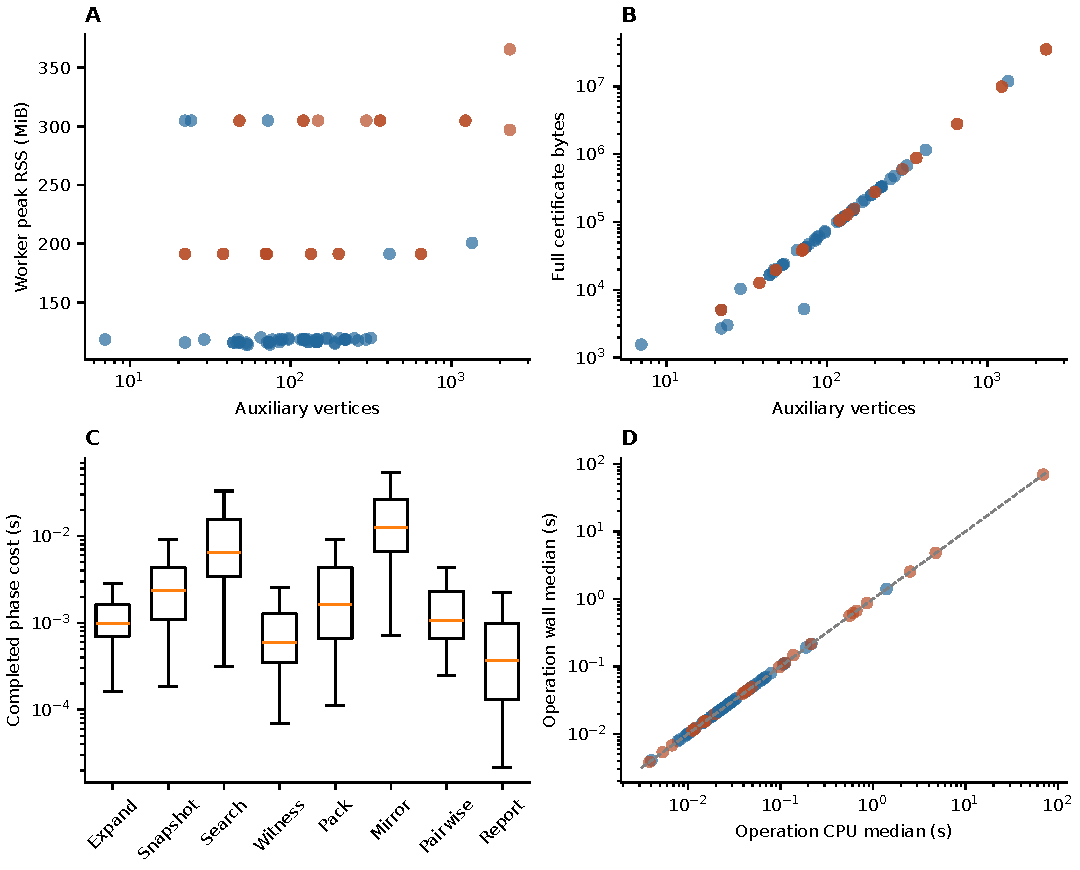
\includegraphics[width=0.98\textwidth]{fig/controlled_stereo_resources.pdf}
\caption{Completed generator-mode resource measurements. (A) Median native
worker peak RSS, including interpreter and imported libraries. (B) Full
certificate size. (C) Per-trial phase distributions; boxes give quartiles,
whiskers use the standard 1.5-interquartile-range rule and outliers are omitted
only from this panel. Pairwise timing covers its declared six-family subset;
report timing serializes the worker's measurement payload. (D) Operation CPU
versus wall medians, excluding interpreter startup. Blue denotes ordinary
cases and orange stress cases. Censored trials are absent from these panels
and retained in Table~\ref{tab:cost-coverage}.}
\label{fig:controlled-resources}
\end{figure*}
